\documentclass[12pt,svgnames]{memoir}
\usepackage[T1]{fontenc}
\usepackage{lmodern}
\usepackage{amssymb,amsmath}
\usepackage{ifxetex,ifluatex}
\usepackage{fixltx2e} % provides \textsubscript
% to include cover page
\usepackage{pdfpages}
% use upquote if available, for straight quotes in verbatim environments
\IfFileExists{upquote.sty}{\usepackage{upquote}}{}
\ifnum 0\ifxetex 1\fi\ifluatex 1\fi=0 % if pdftex
  \usepackage[utf8]{inputenc}
\else % if luatex or xelatex
  \ifxetex
    \usepackage{mathspec}
    \usepackage{xltxtra,xunicode}
  \else
    \usepackage{fontspec}
  \fi
  \defaultfontfeatures{Mapping=tex-text,Scale=MatchLowercase}
  \newcommand{\euro}{€}
\fi
% use microtype if available
\IfFileExists{microtype.sty}{\usepackage{microtype}}{}
\usepackage[margin=1.2in]{geometry}
\usepackage{graphicx}
% Redefine \includegraphics so that, unless explicit options are
% given, the image width will not exceed the width of the page.
% Images get their normal width if they fit onto the page, but
% are scaled down if they would overflow the margins.
\makeatletter
\def\ScaleIfNeeded{%
  \ifdim\Gin@nat@width>\linewidth
    \linewidth
  \else
    \Gin@nat@width
  \fi
}
\makeatother
\let\Oldincludegraphics\includegraphics
{%
 \catcode`\@=11\relax%
 \gdef\includegraphics{\@ifnextchar[{\Oldincludegraphics}{\Oldincludegraphics[width=\ScaleIfNeeded]}}%
}%
\ifxetex
  \usepackage[setpagesize=false, % page size defined by xetex
              unicode=false, % unicode breaks when used with xetex
              xetex]{hyperref}
\else
  \usepackage[unicode=true]{hyperref}
\fi
\hypersetup{breaklinks=true,
            bookmarks=true,
            pdfauthor={},
            pdftitle={},
            colorlinks=true,
            citecolor=blue,
            urlcolor=blue,
            linkcolor=magenta,
            pdfborder={0 0 0}}
\urlstyle{same}  % don't use monospace font for urls
%\setlength{\parindent}{5pt}
%\setlength{\parskip}{6pt plus 2pt minus 1pt}
\setlength{\emergencystretch}{3em}  % prevent overfull lines
\setcounter{secnumdepth}{5}
\usepackage{xcolor}
%theme color
%\definecolor{maincolor}{RGB}{220, 22, 6} %CRIMSON
\definecolor{maincolor}{HTML}{F62459}
%\definecolor{maincolor}{RGB}{70, 61, 140} %DARK SLATE BLUE
\usepackage{framed}
\usepackage{soul}
\definecolor{Light}{gray}{.90}
\sethlcolor{Light}
\newenvironment{quotationb}%
{\color{maincolor}\begin{leftbar}\begin{quotation}}%
{\end{quotation}\end{leftbar}\ignorespacesafterend}
% {\color{white}\begin{shaded}\begin{quotation}}%
% {\end{quotation}\end{shaded}\ignorespacesafterend}
\let\OldTexttt\texttt
\renewcommand{\texttt}[1]{\OldTexttt{\hl{#1}}}
\usepackage{tikz}

%define new chapter style (just for a nicer look)
\makechapterstyle{mystyle}{%
  \chapterstyle{default}
  \renewcommand*{\chapnumfont}{\normalfont\Huge\sffamily\bfseries}
  \renewcommand*{\chaptitlefont}{\normalfont\huge\sffamily\itshape\color{maincolor}}
  \settowidth{\chapindent}{\chapnumfont 111}
  \renewcommand*{\chapterheadstart}{}
  \renewcommand*{\chapnamefont}{\hfill\color{maincolor}\normalfont\Huge\sffamily\bfseries}
  \renewcommand*{\printchapternum}{%
  \begin{tikzpicture}[baseline={([yshift=-.6ex]current bounding box.center)}]
  \node[fill=maincolor,circle,text=white] {\thechapter};
  \end{tikzpicture}\\[1ex]
  \hrule height 1.5pt}
  \renewcommand*{\printchaptertitle}[1]{%
    {\chaptitlefont ##1}}
}

%use new chapter style
\chapterstyle{mystyle}

\author{}
\date{}

\begin{document}


\includepdf{src/content/frontcover/frontcover.pdf}
\addtocounter{page}{-1} % Do not count front cover as page
% Add empty page, not counted in page increment
\null
\thispagestyle{empty}%
\addtocounter{page}{-1}%
\newpage
% \begin{titlingpage}
% 	\centering
% 	
\includegraphics[width=0.5\textwidth]{src/img/eurecom.jpeg}\par\vspace{1cm}
% 	{\scshape\LARGE EURECOM \par}
% 	\textsc{Communication System Security}\par 
% 	\vspace{1cm}
% 	{\scshape\Large Final year project\par}
% 	at Mondeca, Paris\par
% 	\vspace{1.5cm}
% 	{\huge\bfseries A web interface for the Content Annotation Manager\par}
% 	\vspace{2cm}
% 	{\Large\itshape Alessandro Menduni\par}
% 	\vfill
% 	supervised by\par
% 	Anh \textsc{Hyun}\par
% 	Raphael \textsc{Troncy}

% 	\vfill

% % Bottom of the page
% 	{\large \today\par}
% 	\vspace{0.5cm}
% 	Non confidential\par
% \end{titlingpage}

{
\hypersetup{linkcolor=black}
\setcounter{tocdepth}{2}
\tableofcontents
}
\chapter{The context: Mondeca, the product and my
responsibilities}\label{the-context-mondeca-the-product-and-my-responsibilities}

This report concerns the six months I spent as intern at Mondeca, a
French company located in Paris which sells software products capable of
exploiting semantic technologies. In particular, their main product is
the so-called Smart Content Factory (SCF), a complex system that allows
companies to index, annotate and browse through their documentation.
Indeed, main targets of the product are those companies which need to
handle huge amounts of documents (newspapers, legal offices, and so on).

Let's say that National Geographic (who, by the way, is among Mondeca's
customers) wants an automatic way to handle all the scientific articles
it publishes onto its website; this is what it will happen:

\begin{itemize}
\itemsep1pt\parskip0pt\parsep0pt
\item
  it can maintain an ontology with the system
\item
  it may feed SCF with its documents and articles
\item
  SCF analyzes the documents via text mining tools and content
  annotation systems in order to recognize entities inside the text
\item
  the analysis outputs entities detected in the text, entities that have
  been inferred from the text (but that are not mentioned) and
  candidates that could be inserted in the ontology
\item
  a further rule-based classification is possible, meaning SCF will tag
  the documents according to some rules provided by the customer. For
  instance, SCF could tag as ``Not for kids'' the articles that are
  about crime, blood and sex
\item
  finally, it is possible to browse the whole documentation by means of
  a semantic search engine
\end{itemize}

\section{The CAM application}\label{the-cam-application}

What I will be working on is the so-called Content Annotation Manager
(CAM), which is a component of the SCF system. It takes care of text
mining a document, annotating it according to the selected ontology and
yielding out the enriched document. As I enter the company, CAM is just
a step of the process, it is automatically executed and it doesn't have
a UI. Data flows in, data flows out. The only web UI that Mondeca has
for CAM is a poorly presented testing environment (``demo'') that they
demonstrate to potential customers to show off the potential of their
API (which ultimately exposes all the goodness the system produces).
Thus, my role inside Mondeca would be rethinking the current demo UI in
order to provide an easy-to-use, sell-able and pretty web application
that could serve the purpose of both convincing potential clients to
trust the system and allowing them to actually monitor and intervene
over this step of the pipeline.

Here's how it looks like at the moment:

\begin{figure}[htbp]
\centering
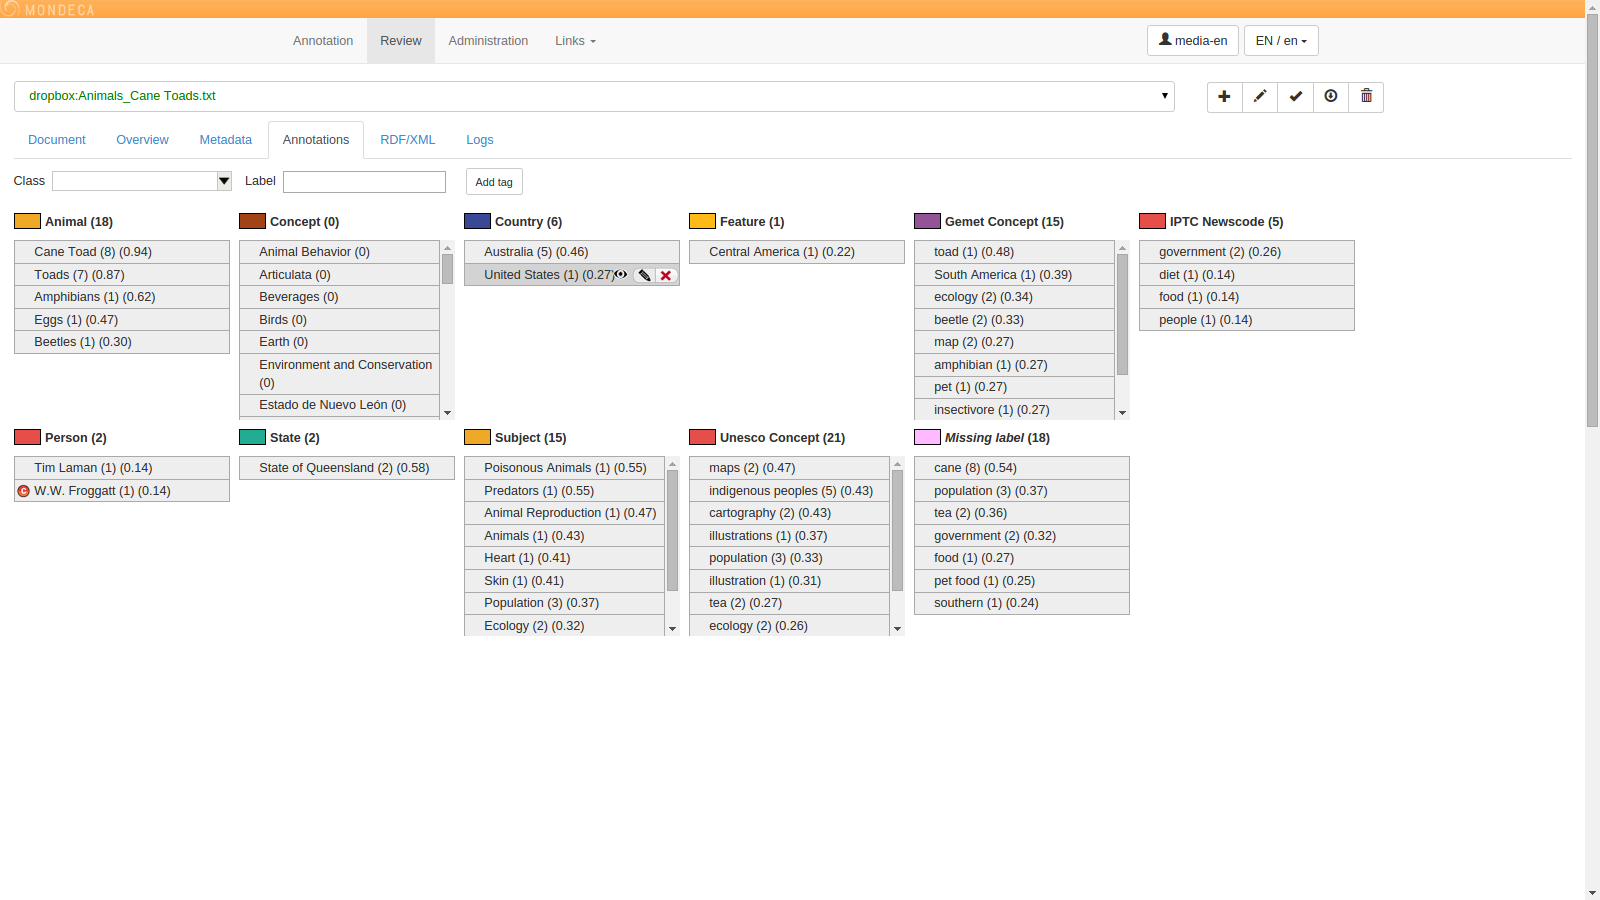
\includegraphics{./src/img/oldCAM-annotations.png}
\caption{Old CAM, Annotations}
\end{figure}

\begin{figure}[htbp]
\centering
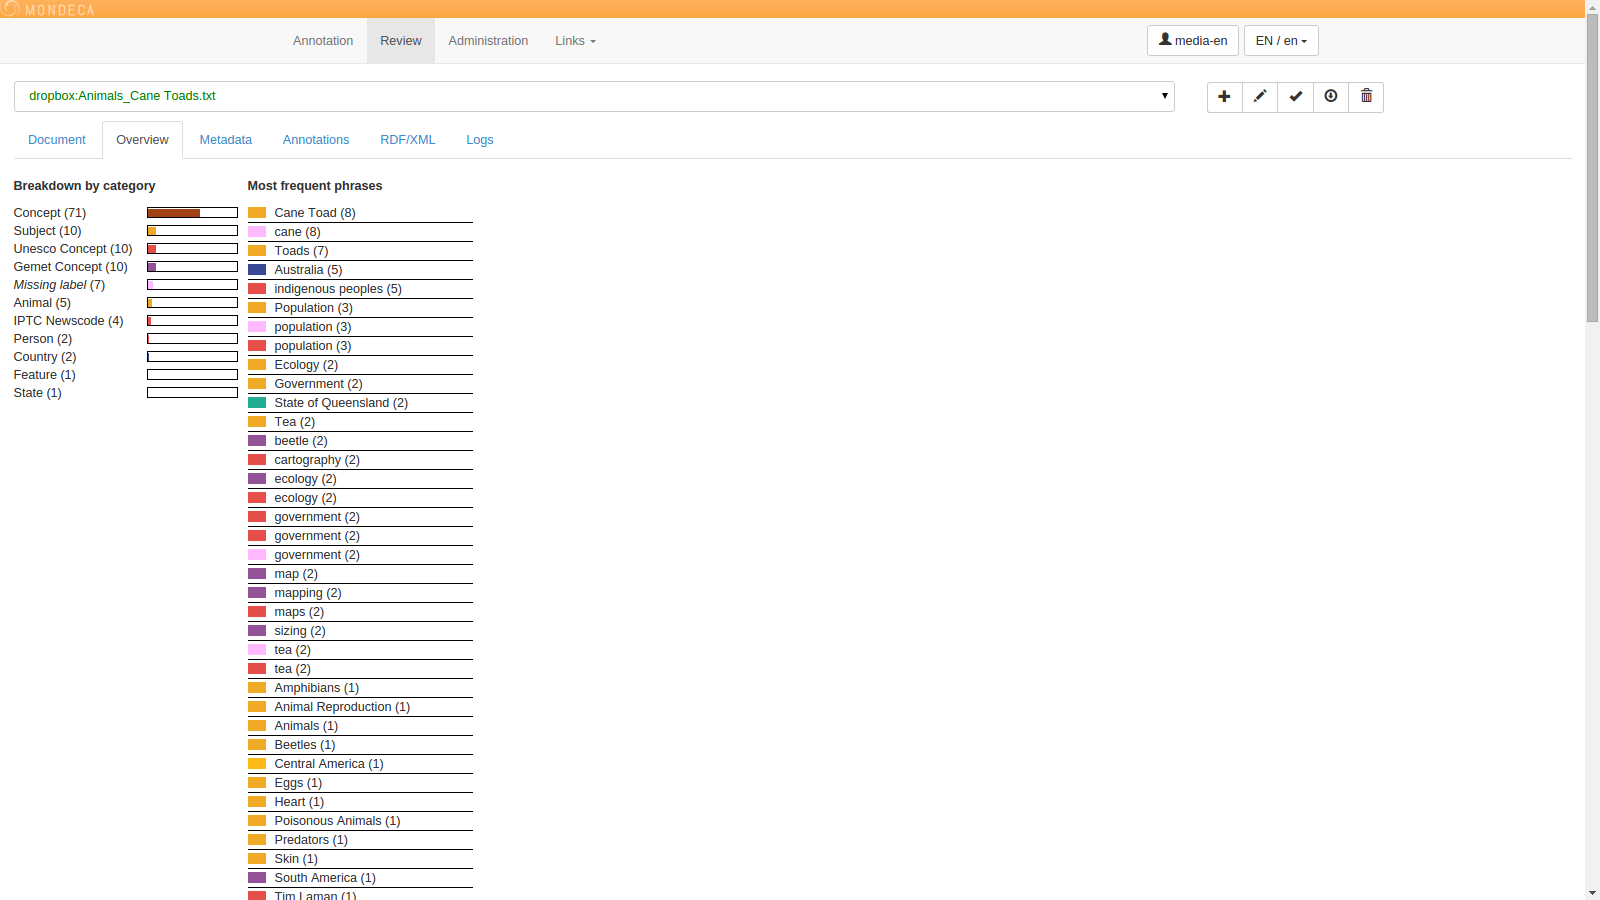
\includegraphics{./src/img/oldCAM-overview.png}
\caption{Old CAM, Overview}
\end{figure}

As it is now, the CAM UI allows the user to do the following:

\begin{itemize}
\itemsep1pt\parskip0pt\parsep0pt
\item
  select resources to be analyzed
\item
  change some configuration settings
\item
  launch the process
\item
  monitor the results
\item
  add and remove annotations
\item
  read the log messages of the system
\item
  read the RDF file that contains all the results of the analysis
\end{itemize}

This is a fairly basic overview of what it can be done but, as I
undertake the challenge of improving the way the user can interact with
the system, I'd rather understand the 10.000 feet view of the product
than diving immediately deep into the details and the nuances of it.
Such a first analysis gives the right vision of what needs to be focused
on, and, most importantly, allows for a clearer conception of what the
underlying servers are capable of producing or doing, in response to
eventual user's requests.

However, the main focus of CAM was better defined during the course of
the iterative process of sketching and validating the ideas with the
team members: while it is mostly used as demo for potential clients at
the moment, the idea is to migrate to a fully fledged app, targeting
those human agents or indexers who are hourly paid to verify and review
automatically assigned tags, bringing on the table their own expertise
on a topic. For instance, a surgeon gets paid to delete wrong tags, add
missing ones and review the general correctness of the analysis of all
the tags related to surgery or body anatomy. The goal becomes then to
help such a kind of users to do their job in as little time as possible;
the challenge is to demonstrate to potential clients that, through the
use of the tools this application provides, human indexers can analyze
many more documents in a given time span, than they would by manually
reading and annotating the text.

\section{Learning about competitors}\label{learning-about-competitors}

During my first days I searched for competing text mining tools with the
purpose of focusing on both the different features they present and the
ways they present their results, in order to take inspiration in terms
of visualization techniques. Such an activity led me to narrow down a
list of very simplified features competitors implement:

\begin{itemize}
\itemsep1pt\parskip0pt\parsep0pt
\item
  Sentiment analysis on entities or keywords
\item
  Sentiment comparisons of a term over different data sources
\item
  Language recognition (e.g.~15\% English 85\% French)
\item
  Part of Speech tagging
\item
  NER
\item
  NED is rarely advertised
\item
  Relevant words occurrence
\item
  Topics/themes (ordered by pertinence)
\item
  Names translation
\item
  Categorization, often times starting from the bunch of documents only,
  without prior knowledge
\item
  Adult content detection
\item
  Documents similarity detection
\end{itemize}

On the visualization side, though, this exercise hasn't been
enlightening: on one hand, existing tools often targets really specific
markets where presentation details aren't taken too much in
consideration, thus the teams working on these solutions focus primarily
on functionalities and ``smartness'' of the software; on the other hand,
data visualization is a highly data-dependent discipline, meaning it is
ultimately based on what type of data one is willing to show and, most
importantly, what kind of reasoning it is trying to support (e.g. -
metrics comparison versus content distribution). For these reasons, I
decided to go on framing the problem CAM is trying to solve for its
users, then to attack eventual visualization challenges from a
completely user-centered perspective, meaning my goal would be finding
the least complex way to guide the user through the possibly big amount
of data the system is capable of producing.

\section{Technical specs}\label{technical-specs}

As it becomes more clear what the scope of the project is, it is common
practice to delimit the work to be done with a series of technical
constraints. In my case, the specifications are pretty loose:

\begin{itemize}
\itemsep1pt\parskip0pt\parsep0pt
\item
  on the \emph{front-end}, HTML, CSS and JavaScript are the technologies
  of choice; the running environment is supposed to include every major
  browser up to the last two versions (Mozilla Firefox, Google Chrome,
  Internet Explorer and Apple Safari), with a minimum supported
  resolution of 1024x768. No particular framework or technology is
  enforced.
\item
  on the \emph{back-end}, the existing code base is written in Java, so
  that is the language of choice. The system already relies on Shiro as
  authentication and security framework, and on JBoss as application
  server.
\end{itemize}

\chapter{The process: technologies, specs and
sketches}\label{the-process-technologies-specs-and-sketches}

In my second month as intern, I went on implementing the initial
sketches that served mainly the purpose of better explaining the ideas I
had for the new version of the CAM application.

\section{Setting up the project}\label{setting-up-the-project}

As it was decided to proceed developing the first two screens, a better
definition of the process to be followed had to be stated. Since I was
working alone on this project, it was decided to slightly change the way
we iterate over the screens, in order to allow me to move both more
quickly and more freely. First of all, after having roughly sketched the
global flow of the application, I should focus on one screen at a time,
completing and validating as many features as possible, before skipping
to the next section. In addition to this, since no other developer is
involved, we decided to reduce the sketching phase, with the goal of
producing semi-working mock ups which are easier to discuss over for
non-technical people. I then adopted the following process:

\begin{itemize}
\itemsep1pt\parskip0pt\parsep0pt
\item
  mock up in the browser a rough representation of a screen
\item
  meet together with the Product Manager and the Sales Manager in order
  to define features and content
\item
  iterate until the screen is finished
\item
  skip to the next screen
\end{itemize}

\section{Choosing the framework}\label{choosing-the-framework}

The first thing to do at this point, was deciding which framework to
adopt so that the development of the functionalities, that enable the
application to offer an interactive experience to the user, will be as
fast and productive as possible. Naturally, an MVC pattern (or similar)
needed to be adopted, as really often happens in web applications and UI
development. I decided to go for Angular, a JavaScript framework
targeting single page applications, after having considered Backbone and
React, as they are the main players in the front-end frameworks game.
While Backbone offers a much more lightweight JavaScript file and great
extensibility and freedom in the choice of plugins, template engine, and
so on, this comes at the cost of having to manually write a lot of code
and browsing through sparse documentation (each plugin has its own). On
the other hand React, the new kid in town, developed by the Facebook's
team and adopted by Instagram.com, is still in its earliest years,
meaning there is not that big of a community yet, plus it somehow
reinvents the way web applications are developed nowadays, requiring a
little bit of effort by people who come from the already-established way
of doing things for the web. So why Angular? There are a lot of reasons
why the decision fell on this framework: first of all, it is really
quick to get going and easy to learn. My first concern in choosing the
right environment, though, was going for solutions that will be easily
maintained by the company when I will finish my stage; people at Mondeca
in fact are prevalently trained in Java programming, and they have in
fact always developed web UIs through the use of the Google Web Toolkit,
which allows them to cross-compile Java code into JavaScript and
HTML/CSS. Thus, I should make it as straightforward as possible for them
to go in and modify something when needed. Plus, a big factor was the
availability for Mondeca of an outsourcing partner which already takes
care of some of the web UI development for them, and which is a huge
expert in Angular-based applications. Therefore, the company can rely on
a trusted partner in the future in order to handle my project's
evolution. However, Angular has a lot of bonus features that are great
for CAM: first of all, it offers out-of-the-box two-ways data binding,
which is the automatic synchronization of data between the model and
view components. The way that Angular implements data-binding lets you
treat the model as the single-source-of-truth in the application. The
view is a projection of the model at all times. When the model changes,
the view reflects the change, and vice versa. This is of course great in
many scenarios, but especially for CAM, which is an application that, at
its core, takes as input a series of tags, lets the user browse through
it and delete some of the tags, then sends as output the outcome of the
user's interactions. In other words, the view needs to simply reflect
what's in the model at all times and each user's decision can be simply
reflected in the model by deleting (or adding) tags to the list. In
addition to this, Angular relies on a declarative way of binding actions
and data to HTML tags, which makes it great for fast and
mock-up-centered iterations, where the design phase is limited and
there's the need for a semi-working mock-up as early as possible in
order to let the Product and Sales Managers be involved in the process.
In fact, since I work alone on the project, I primarily talk with these
people, who are neither designers nor developers, so it's really
important that I allow them to focus on the functionality of the
application, getting rid of static representations of what the final
product will look like. A final consideration on the drawbacks of using
Angular needs to be made: it is a moderately heavy framework that could
suffer from a performance perspective when thousands of bindings are
present at the same time; this is not extremely important for the
typical user that's being targeted by CAM: indeed, the user is supposed
to be on a laptop (no problems related to low-power mobile devices) and
it will certainly be willing to wait for a small initial loading time.

\section{Automate to enhance
productivity}\label{automate-to-enhance-productivity}

It is common knowledge that, in software development, productivity isn't
just related to the time one spends writing down code, rather to the
speed tasks get done at. In order to improve such a metric, good
developers spend some time making their working environment more
ergonomic and smooth; it for this reason that I wish to include in the
following some parts of my job that are not directly related to CAM, but
that allowed me to reduce the burden of side tasks that affect each
developer's everyday job.

\subsubsection*{Front-end}\label{front-end}
\addcontentsline{toc}{subsubsection}{Front-end}

On the front-end side, I made heavy use of tooling and automation, as it
is standard practice today. I relied on \texttt{gulp} as a task runner,
rather than using \texttt{make}, for it exists a huge catalog of
ready-to-use gulp tasks to enhance every single aspect of the developing
activity. What this tool allows to do is basically running standalone
JavaScript code (in other words, JS code that doesn't need a browser to
be run) in a particular sequence through a command-line interface;
moreover, thanks to \emph{watch tasks}, I was able to automatically run
my sequence at every saved modifications to my source files. In
particular, it was taking care of:

\begin{itemize}
\itemsep1pt\parskip0pt\parsep0pt
\item
  concatenation, vendor-prefixing and minification of CSS files
\item
  concatenation, uglification and linting of JS files
\item
  minification and in-lining of HTML templates
\item
  compression of images
\end{itemize}

More on these techniques in Chapter 5. In addition to tasks automation,
another area in which tools can improve programmers' life is dependency
management; I used \texttt{bower} to manage JavaScript and CSS
libraries, and \texttt{npm} to manage NodeJS modules, like
\texttt{gulp}'s tasks and external tools. It is especially useful to
rely on such tools when cooperating with other people, since they can
easily set all the tooling up and fetch all dependencies by simply
downloading the source and running the install scripts:
\texttt{npm install \&\& bower install}.

\subsubsection*{Back-end code and
deployment}\label{back-end-code-and-deployment}
\addcontentsline{toc}{subsubsection}{Back-end code and deployment}

On the back-end, I already had some Maven tasks to run that were coming
from the existing project I inherited. So I simply made compilation and
deployment on test server a single job, by creating a \texttt{Makefile}.
However, such an activity takes several seconds (up to 40s on my
laptop), which can be a problem, especially when testing small changes,
since long waits may interrupt the mental flow. I thus decided to divide
deployment step into two parts, that don't need to go together all the
time:

\begin{itemize}
\itemsep1pt\parskip0pt\parsep0pt
\item
  deployment of back-end code, which consists in copying the WAR file
  into the server
\item
  deployment of front-end code, which I could speed up by an incredible
  amount by simply treating the WAR archive as a simple RAR archive, and
  substituting modified files; this made front-end code's deployment as
  fast as half a second
\end{itemize}

\subsubsection*{Version control systems}\label{version-control-systems}
\addcontentsline{toc}{subsubsection}{Version control systems}

Finally, I set up a versioning system for both front-end and back-end.
On the back-end, I kept using \texttt{svn} which is the system of choice
at Mondeca, and allows developers to synchronize their project with the
internal integration system (Jenkins). On the front-end, I decided to
use a local \texttt{git} repository, in order to benefit of local
branching and smarter changes history.

\section{Framing the problem: specs}\label{framing-the-problem-specs}

In order to get a deeper knowledge of the current state of the
application, and to start forming an idea of the desired state of the
next version of it, I iterated through a series of sketches; this phase
is of the uttermost importance since, by showing concrete drawings of
what I think it would be great to show and to hide to the team members,
I have the possibility to learn about the product itself. Every team
member has something to add to the design phase, since everyone of them
is expert in a particular side of CAM (current UI, back-end
architecture, system's capabilities, gotchas, and so on). Thus,
iteration after iteration, I kept putting together all this knowledge
and refining my ideas, until a complete picture of where CAM is now and
where it's going next was ready. The next fundamental thing to do then
is discussing my ideas with both the Product Manager and the Development
Team Leader, in order to collect their feedback and finally redacting a
draft of the requirements document, so that the developers, the managers
and me could agree on a list of feature to implement. This isn't by any
means trying to be a finalized and frozen document, but at the contrary
it acts as a reference people can refer to while pushing the product
forward.\\The result of such a cyclic process, can be trusted here as a
way to better define the main purpose of the application and its core
sections; let's quickly go through it, keeping in mind that not all the
listed features made it to the final realization of the application
(especially in the troubleshooting and user sections, which got moved
out of scope during the course of the project).

\subsection{Main purpose of the
application}\label{main-purpose-of-the-application}

The purpose of the CAM web application is allowing the user to load one
or more resources and visualize the result of the analysis process. The
user will need to see an high-level overview, and a detailed view of the
analysis, one document at a time. In addition to this, privileged users
will be capable of browsing the log messages and the actual RDF file
that comes out of the processing pipeline.

\subsection{Core sections}\label{core-sections}

In order to properly group up the elements of the application, the
following sections will be present:

\begin{itemize}
\itemsep1pt\parskip0pt\parsep0pt
\item
  File selection
\item
  Overview
\item
  Review
\item
  Troubleshooting
\item
  User profile
\end{itemize}

\subsubsection*{File selection}\label{file-selection}
\addcontentsline{toc}{subsubsection}{File selection}

This section allows the user to select which files she wants to send to
the analysis process. A pool of files coming from different sources is
created, shown under the form of a list.

Such sources can be

\begin{itemize}
\itemsep1pt\parskip0pt\parsep0pt
\item
  Manually inserted text
\item
  Dropbox
\item
  Locally stored file (on the client's machine)
\item
  Remotely stored file (via URL)
\end{itemize}

The list of files presents, for every file, the following information:

\begin{itemize}
\itemsep1pt\parskip0pt\parsep0pt
\item
  name of the file
\item
  type of the file
\item
  workflow to be used
\item
  source of the file (e.g. - Dropbox)
\end{itemize}

The user can ``check'' files that she wants to

\begin{itemize}
\itemsep1pt\parskip0pt\parsep0pt
\item
  remove from the pool
\item
  associate with a workflow
\item
  run
\end{itemize}

The user can:

\begin{itemize}
\itemsep1pt\parskip0pt\parsep0pt
\item
  remove a file from the pool
\item
  check all
\item
  uncheck all
\item
  run all
\end{itemize}

While the process is running, the user can keep track of the progress.
Both per file progress and global progress.

\subsubsection*{Overview}\label{overview}
\addcontentsline{toc}{subsubsection}{Overview}

This section looks and feels as a normal dashboard, and it aims at
showing the following measures:

\begin{itemize}
\itemsep1pt\parskip0pt\parsep0pt
\item
  title of the document
\item
  workflow selected
\item
  number of words analyzed
\item
  number of tags generated
\item
  number of seconds needed to process that document
\item
  metadata of the document, them being

  \begin{itemize}
  \itemsep1pt\parskip0pt\parsep0pt
  \item
    customer's decision
  \item
    as many as the customer likes
  \item
    as different in type as needed
  \end{itemize}
\item
  composition of the generated tags, broke down by quality, meaning
  whether they have been

  \begin{itemize}
  \itemsep1pt\parskip0pt\parsep0pt
  \item
    detected in the text
  \item
    inferred
  \item
    suggested as candidates
  \item
    generated as rule-based tags
  \end{itemize}
\item
  composition of the generated tags, broke down by taxonomy
\item
  rule-based tags
\item
  main topic the document is about, exploiting a side-effect of a
  cluster-based scoring algorithm already in use
\item
  top 3 subtopics with metric, if any (e.g. ``the document is also
  partly about HEALTH 20\%, FINANCE 10\% and ANIMALS 8\%'')
\end{itemize}

The UI has a tiled layout, meaning it is composed of rectangles, each
one of those containing a measure or a piece of information.
Composition-type measures are presented under the form of pie charts.

\subsubsection*{Review}\label{review}
\addcontentsline{toc}{subsubsection}{Review}

This section allows the user to browse through the entities that have
been found or generated. It is logically divided into two main parts:
filters and results. In addition to these two, another feature is new
tags addition: the user can add a new tag (that was missed by the system
or that's missing in the taxonomy). This may happen in two ways:

\begin{itemize}
\itemsep1pt\parskip0pt\parsep0pt
\item
  by the add tag button
\item
  by selecting a word in the text and right clicking it
\end{itemize}

The process of adding the tag unfolds itself in the following steps:

\begin{itemize}
\itemsep1pt\parskip0pt\parsep0pt
\item
  type in the new tag
\item
  select its class from a intelligently filled list
\item
  suggest the class if it's missing in the taxonomy
\end{itemize}

\paragraph*{Review: Filters}\label{review-filters}
\addcontentsline{toc}{paragraph}{Review: Filters}

Filters allow the user to narrow down the quantity of information that
it is displayed in the results section. Filters are:

\begin{itemize}
\itemsep1pt\parskip0pt\parsep0pt
\item
  score
\item
  class
\item
  quality, being it

  \begin{itemize}
  \itemsep1pt\parskip0pt\parsep0pt
  \item
    detected
  \item
    inferred
  \item
    candidates
  \item
    rule-based
  \end{itemize}
\end{itemize}

Filters are meant to be collapsible into a side bar which disappears on
the left-hand side of the screen. The filters bar itself is structured
in a way that it allows the different filters to be collapsed or
expanded, in a tree-fashioned style. This allows for further addition of
filters.

\paragraph*{Review: Results}\label{review-results}
\addcontentsline{toc}{paragraph}{Review: Results}

The results are simply 2 different views of the same knowledge:

\begin{itemize}
\itemsep1pt\parskip0pt\parsep0pt
\item
  selected entities in a list
\item
  selected entities in the text
\end{itemize}

The list of entities shows, for every entry, the following information:

\begin{itemize}
\itemsep1pt\parskip0pt\parsep0pt
\item
  name
\item
  taxonomy
\item
  occurrences
\item
  score
\end{itemize}

The text view displays the document itself and, via highlighting or
underlining, it allows the user to locate the selected entities in the
text itself.

\subsubsection*{Troubleshooting}\label{troubleshooting}
\addcontentsline{toc}{subsubsection}{Troubleshooting}

This section targets privileged users, who need to read through log
messages and browse the whole RDF file which contains the result of the
analysis. It is therefore subdivided in two sections:

\begin{itemize}
\itemsep1pt\parskip0pt\parsep0pt
\item
  RDF
\item
  Log
\end{itemize}

\paragraph*{Troubleshooting: RDF}\label{troubleshooting-rdf}
\addcontentsline{toc}{paragraph}{Troubleshooting: RDF}

The RDF file is split in Valid and Invalid RDF, by means of tabs. Both
valid and invalid RDF is further split into three chunks:

\begin{itemize}
\itemsep1pt\parskip0pt\parsep0pt
\item
  metadata RDF
\item
  knowledge RDF
\item
  occurrences RDF
\end{itemize}

The user can decide which one she wants to read through buttons.

The RDF code is displayed in a researchable area: the user can search
for a particular word, or tag, and go directly to that part of the code.
Tags in the code will allow collapsing and expanding actions, as in
regular text editors.

\paragraph*{Troubleshooting: Log}\label{troubleshooting-log}
\addcontentsline{toc}{paragraph}{Troubleshooting: Log}

The log messages are displayed in a table containing the following
fields:

\begin{itemize}
\itemsep1pt\parskip0pt\parsep0pt
\item
  module name
\item
  message type (INFO or ERROR)
\item
  referenced entity
\item
  message code
\item
  processing time
\item
  date
\item
  time of the day
\item
  presence of a stacktrace (YES or NO)
\end{itemize}

In case a stacktrace is present, clicking on ``YES'' will lead to a view
showing:

\begin{itemize}
\itemsep1pt\parskip0pt\parsep0pt
\item
  relative message's details
\item
  stacktrace
\end{itemize}

By means of a button, the user can switch between the ``table view''
displaying all the messages and the ``time view'', which breaks down
modules by time. This allows the user to understand which parts of the
pipeline took the most time, and which parts are the most efficient.

\subsubsection*{User profile}\label{user-profile}
\addcontentsline{toc}{subsubsection}{User profile}

This section is still to be defined.

My suggestions for it would be:

\begin{itemize}
\itemsep1pt\parskip0pt\parsep0pt
\item
  user's permissions

  \begin{itemize}
  \itemsep1pt\parskip0pt\parsep0pt
  \item
    can the user access all the files?
  \item
    can the user access all the workflows?
  \item
    can the user access the troubleshooting section?
  \end{itemize}
\item
  create, edit, delete workflows
\item
  change language
\item
  in the future, past sessions
\end{itemize}

\section{The first mock-up}\label{the-first-mock-up}

After agreeing on the screens, I started to mock up in HTML a static
version of the overview page, so that it can be seen how it looks like
in the browser. Moreover, it allows the Team Leader and me to start
thinking of the theming of the application, phase which usually gets
skipped in the sketching process. My first day of mocking up saw me
transforming this sketch

\begin{figure}[htbp]
\centering
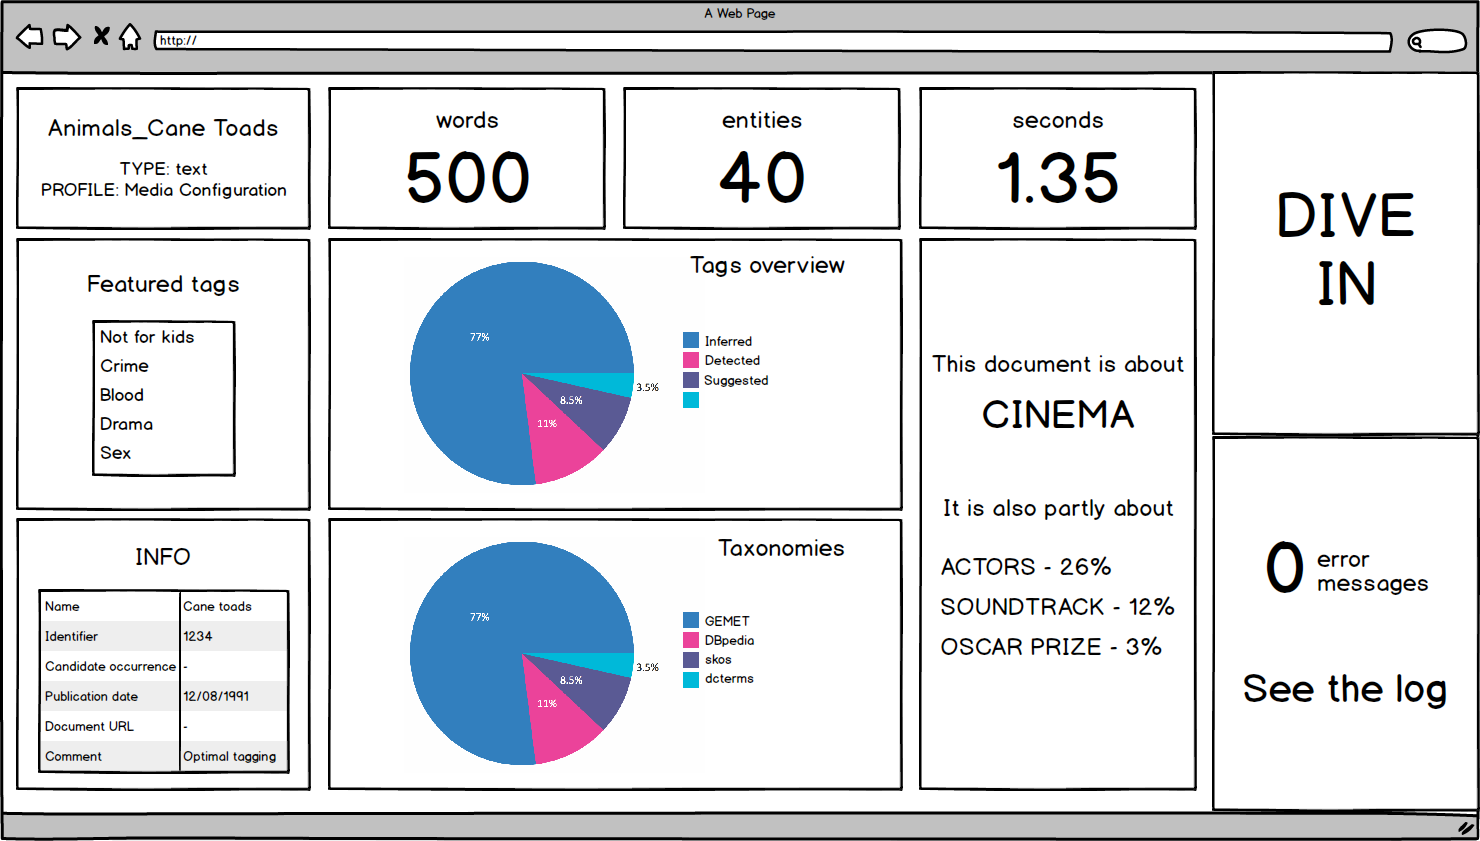
\includegraphics{./src/img/sketch-overview.png}
\caption{Sketch, Overview}
\end{figure}

into this HTML page

\begin{figure}[htbp]
\centering
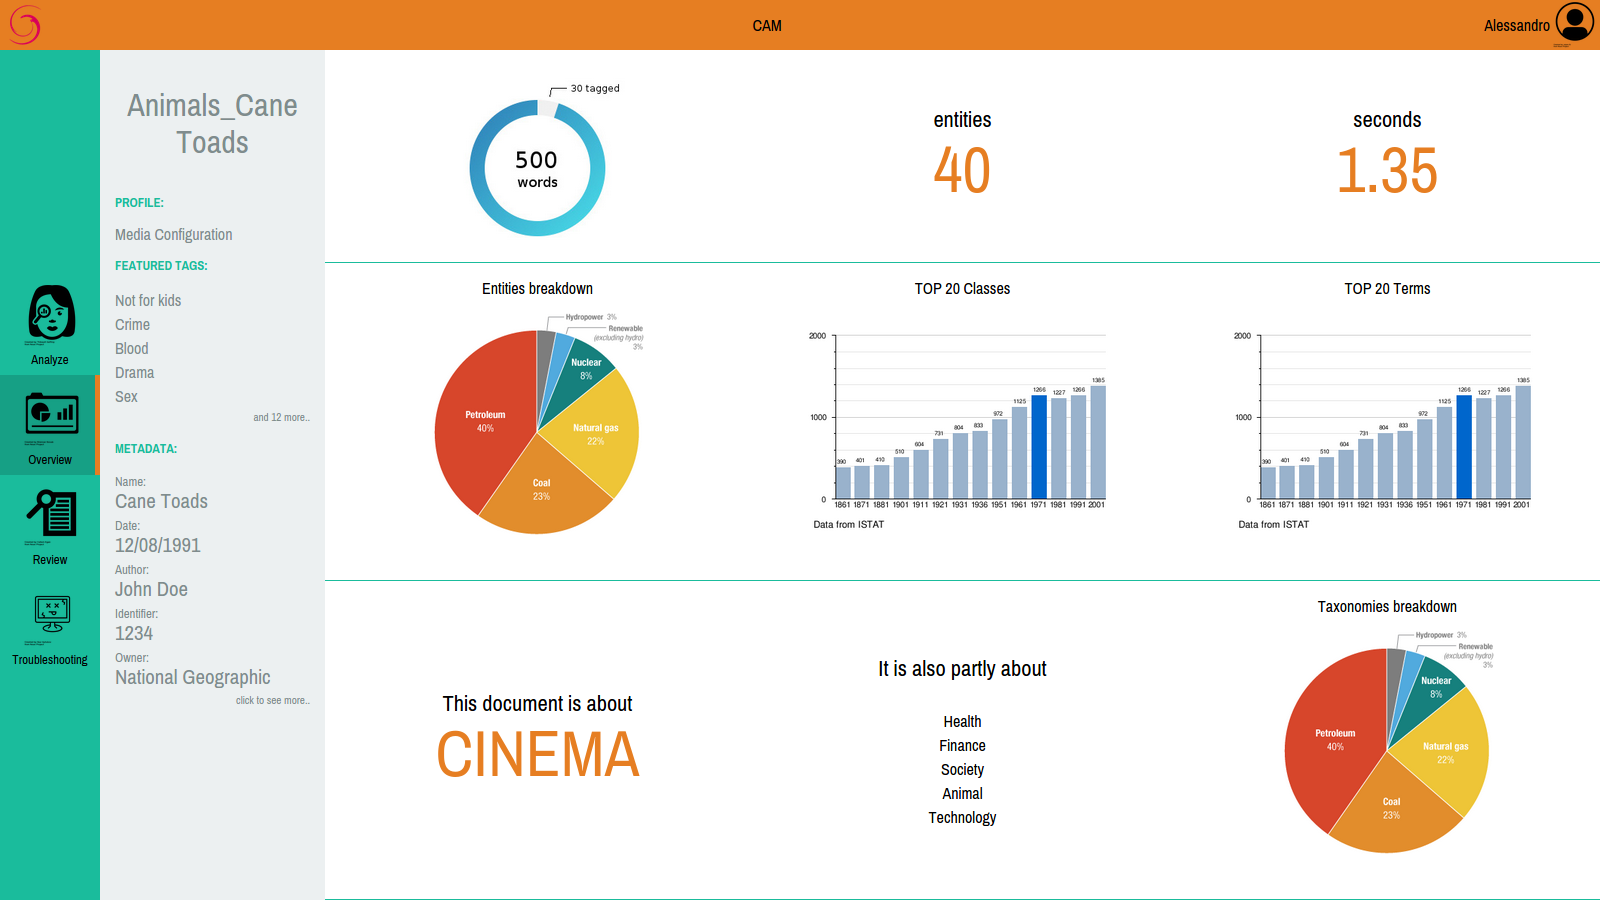
\includegraphics{./src/img/mockup-overview.png}
\caption{Mockup, Overview}
\end{figure}

\chapter{The core screens}\label{the-core-screens}

In the following chapter, I commit to describe the most important
screens of the application, trying to convey both the intended use and
the reasoning behind those, which led to the conception of the layout.
In other words, my intention is to describe the functionalities of the
various parts of the application, while focusing on design decisions.
The order of the exposition follows the chronological order in which
they were validated and developed through the course of the project.

\section{Overview}\label{overview-1}

The first screen I focused on is the ``overview`` screen, which is the
landing page the user is redirected to after the analysis of a document
has completed. The goal is to provide the user a quick glimpse of the
most important results of the text mining and content enrichment
process, while showing measures that could give some hints about what
could be a good course of action from that moment on; so for instance,
an administrator could look at this screen and be immediately aware of
how good the underlying taxonomy is, whereas a human agent can see if
there's something obvious to do, like wrong automatic deletions of tags,
or irrelevant terms that shouldn't appear in the most relevant terms
list. Selecting the right quantity and type of information to display in
this screen was tricky, since there was the need of containing
everything in a single screen (no scroll allowed) while providing
meaningful insights to both administrators (who primarily care about
taxonomy's quality and annotating system's performance) and human
indexers (who would like to be helped in the process of understanding
what happened during the analysis and what can be easily fixed). For
these reasons, my design includes just 9 ``widgets'', organized in 3
rows, so that every piece of information is effortlessly reachable by
the eye, being it widely separated by blank space from the other
elements of the page. Measures and, more generally, data about the
document, are grouped in a logical manner: on the left-hand side,
``wordy'' descriptive information is presented, such as metadata on the
document itself, number of words analyzed, configuration settings
applied to the pipeline in order to process this resource (mainly a list
of the taxonomies involved and whether or not the content classifier was
enabled). On the right-hand side, the real dashboard-like content, laid
out top to bottom from most informative to most general. As we can see
in the screenshot, in the first row I decided to put information that is
widely related to the aboutness of the document itself, being it a
high-level dissection of the main topics it touches, plus a sequence of
tags produced by the underlying classifier, which is capable of spotting
existing relationships between elements that come from the global
knowledge, which it is formed over the document's content: what this
means is that, basing on some rules configured by the customer, the
system can classify the document putting together both what it has been
found in the text, and what it has been inferred by means of the
taxonomy.

\begin{figure}[htbp]
\centering
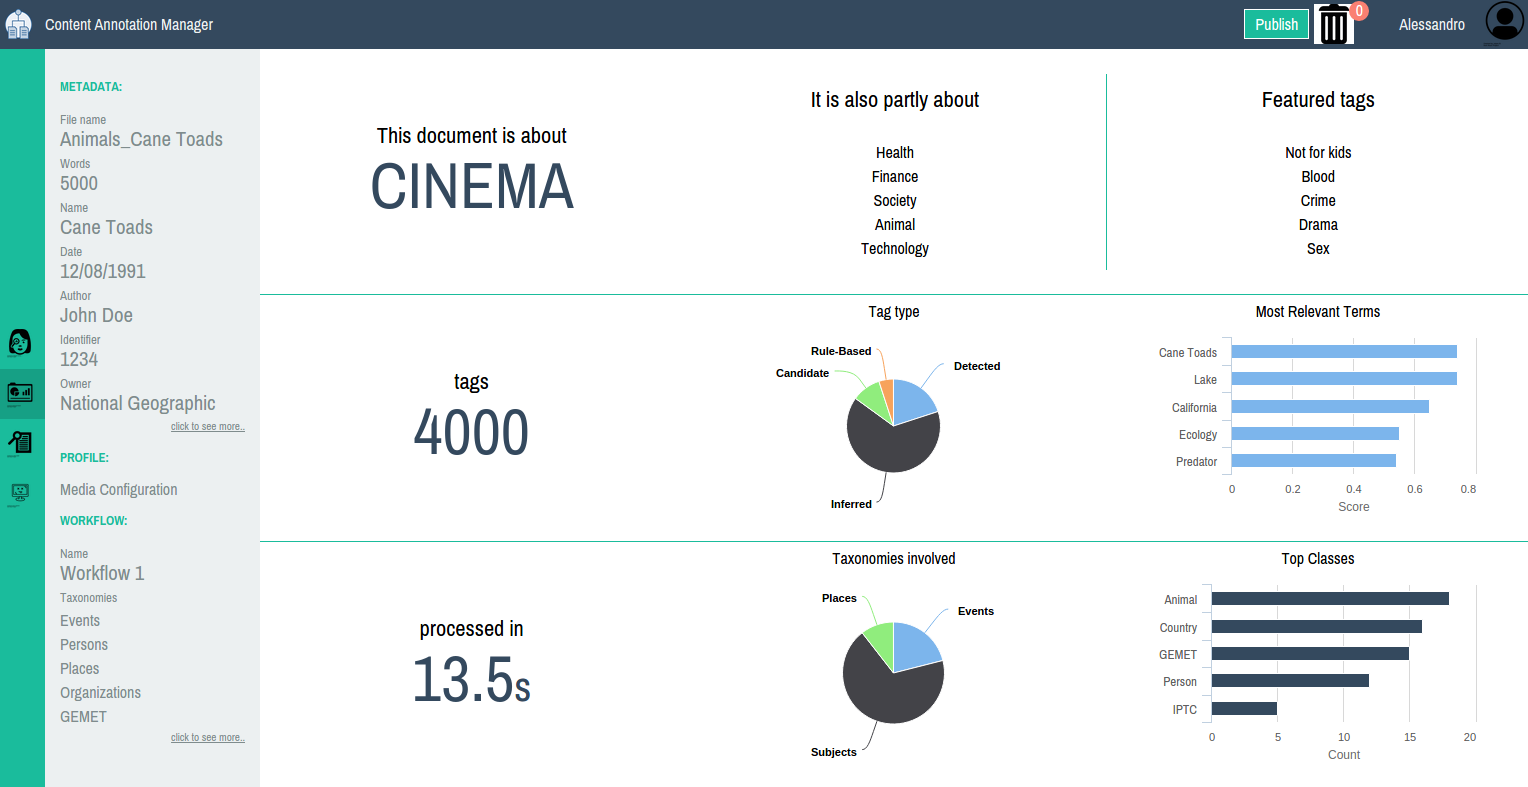
\includegraphics{./src/img/overview-A.png}
\caption{Overview screen, version A}
\end{figure}

So, in the example in the picture, the classifier was able to determine
that a given article can be identified as ``Not for kids'' basing on the
presence of ``adult'' terminology, content or topic. What it's
interesting here, is that the Web API doesn't - yet - provide the list
of ``main topics'', as I called them in my mock-up; the idea of showing
this incredibly useful and insightful piece of information came from a
discussion that I had with the Sales Manager and one of the core
back-end developers of the team. This developer was briefly explaining
an algorithm he personally invented to score entities found in the text,
by means of clusters. What we realized is that, since the fundamental
nature of the model they're using is tree-like, meaning there's always
available a broader-narrower relationship between resources that allows
to bring the model down to a tree, this algorithm can always represent
entities detected in the text and their relationships in a way that
allows to split such a tree in clusters. By clustering together
different entities under a cluster's root node, the system will easily
output relevancy scores for the given terms; thus, in a document
presenting a big cluster having as root node the ``health'' term, and a
small cluster having as root ``finance'', a term belonging the first
cluster will be considered as ``more relevant'' than a term belonging to
the second cluster, by weighing more occurrences of the former than
occurrences of the latter. The really interesting notion here is this
clustering process, that seems to perform very well and which gives out
some interesting analysis of the content of the resource being analyzed;
however, clusters are just a step of the whole algorithm, and they are
not stored anywhere, nor kept in memory after scoring completes. What my
design is suggesting is to revisit the already existing software so that
this clusters can be sent to the client application. I strongly believe
that this is really useful for CAM, especially when we are thinking of a
dashboard, aiming to give the most concise summary of what the
annotation process has done, with respect to what's actually present in
the text. What follows in the screen is somehow more ``standard''
statistics: in the second row, I put the total number of words analyzed,
which is important in order to correctly interpret what follows, a
breakdown of all the tags by type, or category, answering to questions
like ``how many of the tags that we have are coming from the text?'',
``how many of those have been inferred by the system?'' and so on.
Finally, the top 5 most relevant terms, organized in a bar chart. The
third and last row contains measures that are not less important, yet
they are placed in the bottom area of the screen, since they are somehow
less related to the document itself, but rather more to the quality of
the system and of the model. In fact, here the user can find a timing
estimate of how long the process was, a breakdown by taxonomies that
were involved in the pre configured workflow (which complements the
lists already shown in the sidebar, since it's very likely that not all
those taxonomies actually yielded out some term) and the top 5 most
frequent classes. In such a way, administrators or taxonomists can
visualize which taxonomy is useful and which is not, which classes are
always triggered and which ones are probably not that important in the
business model of their company. In conclusion, there is another
important thing to notice about this first Overview screen: the whole
aboutness row relies on the presence of two plugins, the cluster-based
scoring plugin and the rule-based classification plugin. But, as things
are now, it is entirely up to the customer to configure those plugins
and drop them into their pipeline. What this implies for the design of
the screen is that we could not have the first row, since the data it
depends on could not be available. The solution for this was designing a
``plan B'', introducing a new row, that shows three highly correlated
charts: the most relevant terms, as it is already shown in the original
version, the most frequent terms, which is basically the same chart
ordered by occurrences, and the most frequent AND relevant terms, which
is a combination of both the previous charts. These three graphics, when
compared with one another, tell the user much a deeper story about the
terms that are found in the text, thus forming a great fallback in
absence of the ``aboutness'' data.

\begin{figure}[htbp]
\centering
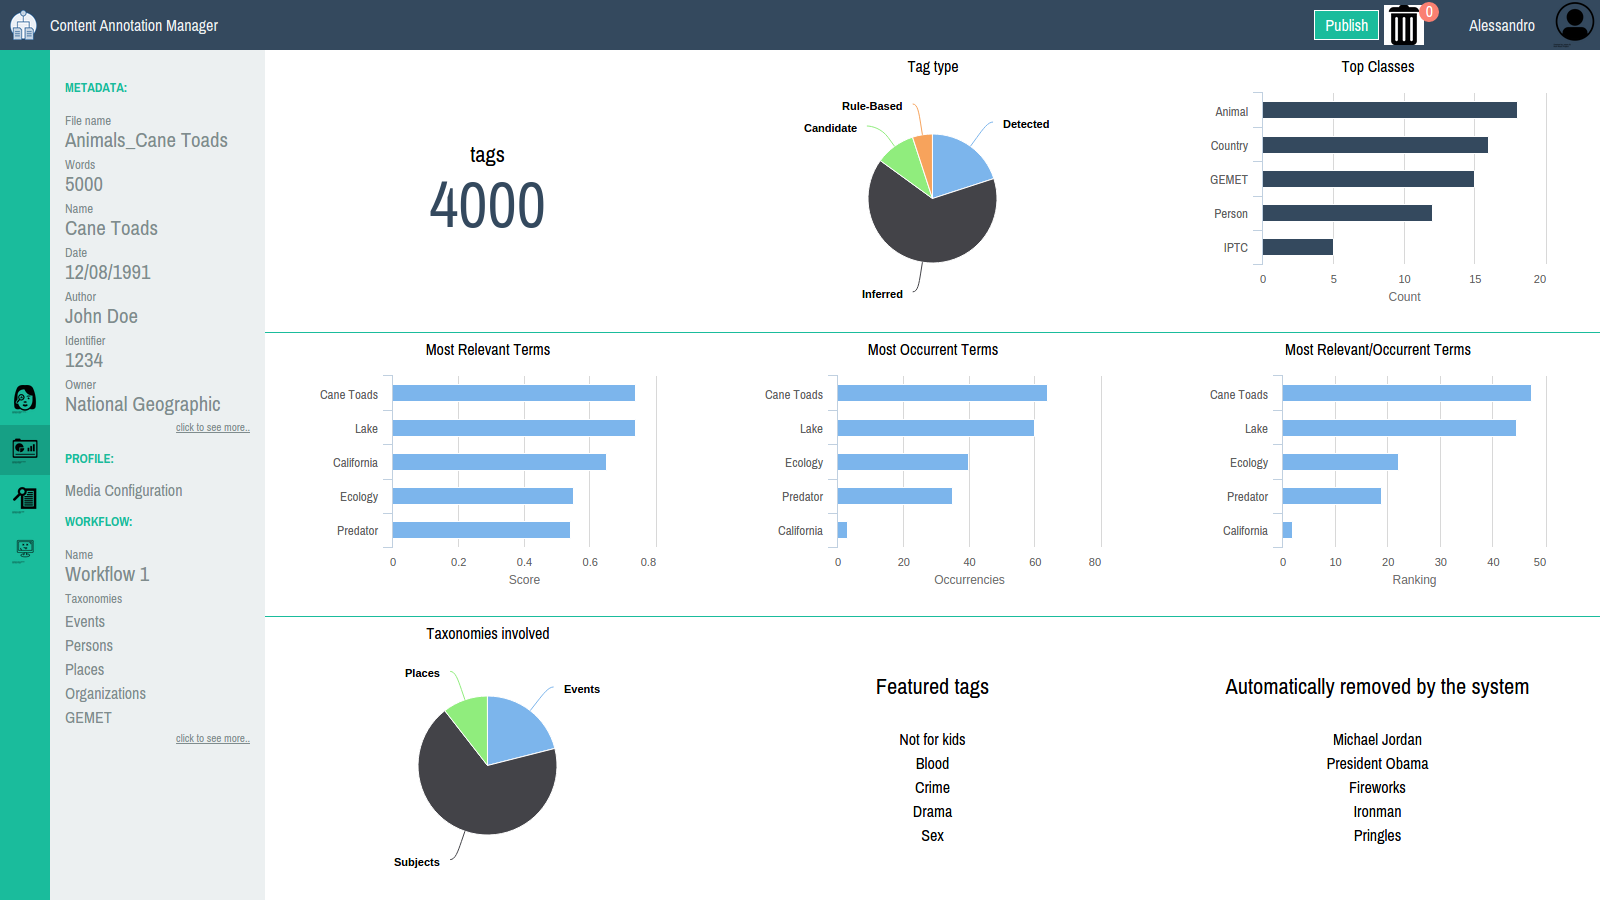
\includegraphics{./src/img/overview-B.png}
\caption{Overview screen, version B}
\end{figure}

\section{Review}\label{review-1}

Regarding the ``review'' screen, its main goal is to enable the users to
quickly browse through a possibly very long list of tags, understand the
logic that made the system annotate the document with those tags and, in
case she considers some annotation wrong, remove one or more particular
tags. Moreover, whenever the user realizes that an important tag is
missing, either because it wasn't detected in the text or because she
thinks it's correlated and useful to the company owning the content, she
can add it: let's say, an article covering some aspect of Michael
Schumacher's life, but never mentioning F1, can still be annotated with
a ``F1'' tag by a human agent, in case this couldn't be automatically
inferred by the system. With these objectives in mind I approached the
design of this screen from the user's point of view entirely. In order
to better express how I did this, let's rely on a user story:

\begin{quotationb}
``a human agent expert in some given area is provided with a list of
already annotated documents to verify and review, being paid basing on
the throughput of documents''
\end{quotationb}

Having a user story, no matter how brief and straightforward it may be,
is powerful way to stay focused on what the user's needs and goals are;
in fact, since I knew from the beginning what the final experience of my
targets should be, I could concentrate on what really matters to them.
My idea is to get rid of every static representation of the outcome of
the analysis, and to allow people to narrow down the amount of
information they are presented with letting them focusing on the
possibly few annotations they are interested in. In order to achieve
this kind of user experience, I provide two simple yet powerful tools: a
table of tags and some filters. By using the filters, a human indexer
can easily see only the tags she is supposed to review and get her job
done in the smallest amount of time possible; moreover, by making good
use of the high-level information she has just seen in the Overview
screen, quick action can be immediately taken, without having to spend
too much time digging into the text, details, comparisons, and so on. At
this point, I was more than ever decided to go for a single-page web
application: it doesn't feel right to have to refresh the page every
time the user hits on a filter, as it usually happens in the
competitor's' tools; for this reason I feel like adopting a heavy
client-side framework like Angular was the right call. The third most
important element of a UI of this kind is, of course, the original text,
and the context in which detected terms are found: in other word, it is
important to have access to the position in the text where an entity
lives, so to not only be able to recognize whether or not the annotation
was correct, but also to understand why an element appears on the list
(it happened in the past of not understanding why there was a ``bear''
in the list, because the system simply normalized the past participle
``born'' into ``bear''; in such cases, it's extremely important to be
able to track back to the analyzed text). In order to address this, I
decided to split the screen into two equally sized columns, one
containing the table of tags, the other containing the annotated text,
while hiding behind a toggle button a drawer panel containing the
filters. A further adjustment to the design that I made was not
overlaying the panel to the two columns, rather ``pushing'' the content
to the right, basically displaying simultaneously on the page three
columns: filters, tags and text. This was done with the goal in mind of
allowing the user to see what's changing in the list and in the
annotated document, as she filters out entries; and this is made
especially important by the interactive nature of the application I set
out to build, since it would be useless to have a single-page web
application, capable of instantaneously react to user's input, if the
filters' bar covered partially the resulting outcome of those actions.

\begin{figure}[htbp]
\centering
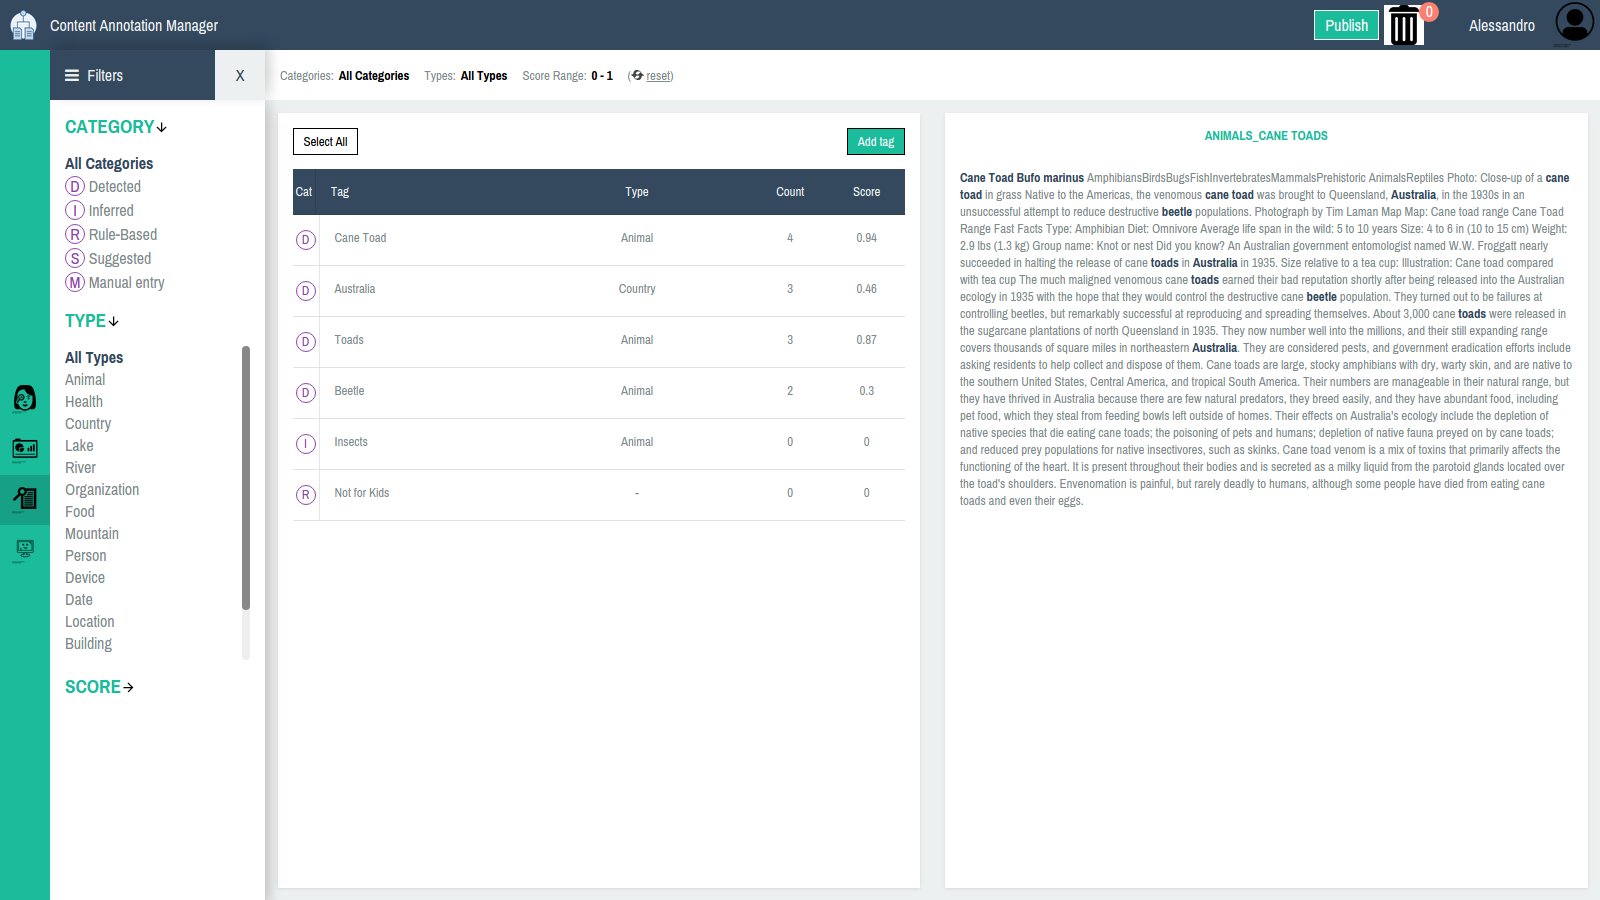
\includegraphics{./src/img/review-open.png}
\caption{Review screen, filters open}
\end{figure}

Finally, always along the lines of helping a human agent do her job
quickly and promptly, I added breadcrumb faceted navigation on top of
the screen, to help the user keep track of what filters are enabled, at
any given time. This may seem a strange decision, since there's no
actual hierarchy in the filtering process, but it is still useful to
have it as a feature in the app, since we don't want CAM's users to
validate tags just because they forgot that something can be out of the
list that's on the screen in that moment. This also gave me a chance to
put a ``reset filters'' button in a place where it could be intuitive
for the user to find it.

\begin{figure}[htbp]
\centering
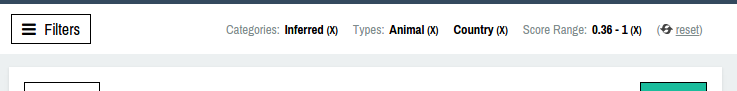
\includegraphics{./src/img/review-breadcrumb.png}
\caption{Review screen, breadcrumb faceted navigation}
\end{figure}

\section{Analyze}\label{analyze}

Introducing the ``analyze'' screen (in lack of a better name). This
screen is probably going to be the first one that the users are going to
interact with: indeed, it contains the core controls which enable them
to choose the resources to submit to the analysis process, see the
progress of said analysis and then dive into the results for the
selected resource. Moreover, here one can change some of the workflow's
parameters: remove some taxonomies from the list of the ones that will
be used, disable the classifier or specify which rules should it take
into account during its classification process (which is, indeed,
rule-based). In order to design a solution for all of these tasks, I
decided to split the needs the user might have in two sections: on one
hand there is the resource selection, which should include buttons to
add files/resources, a list of the selected ones, a way to change the
parameters, and so on; on the other hand, there is the process
monitoring, which should provide visual feedback for the user, such as
an indication of how long the process will take, which resources have
already been processed, and so on. After having done this, I tackled the
design challenges and, through a sequence of iterations, I came up with
a solution composed by the following elements:

A sidebar, on the left-hand side of the page, visually representing the
process monitoring section; it includes, from top to bottom: a button to
perform the most important action - running the analysis on all the
selected resources an overview of the work already done and yet to be
the global progress (e.g. - 40\% completed) some statistics on the
results of the review of the documents performed by the user itself
(e.g.~removed tags) The choice of having a sidebar comes from two
considerations: first, it is consistent with the general design of the
application, which presents a sidebar in almost every section, and
secondly, it makes perfect sense to logically separate the ``action'',
displaced in the main area of the page, from the ``details''. From a
design point of view, grouping is the technique I relied upon the most
in order to visually represent the relationship existing among the
various pieces of data. In fact, by doing this, it becomes obvious that
what's going to appear and change on the left, is just an addition, or
an extra if you will, to what occupies the main portion of the screen,
which instead is the most important thing to pay attention to.

\begin{figure}[htbp]
\centering
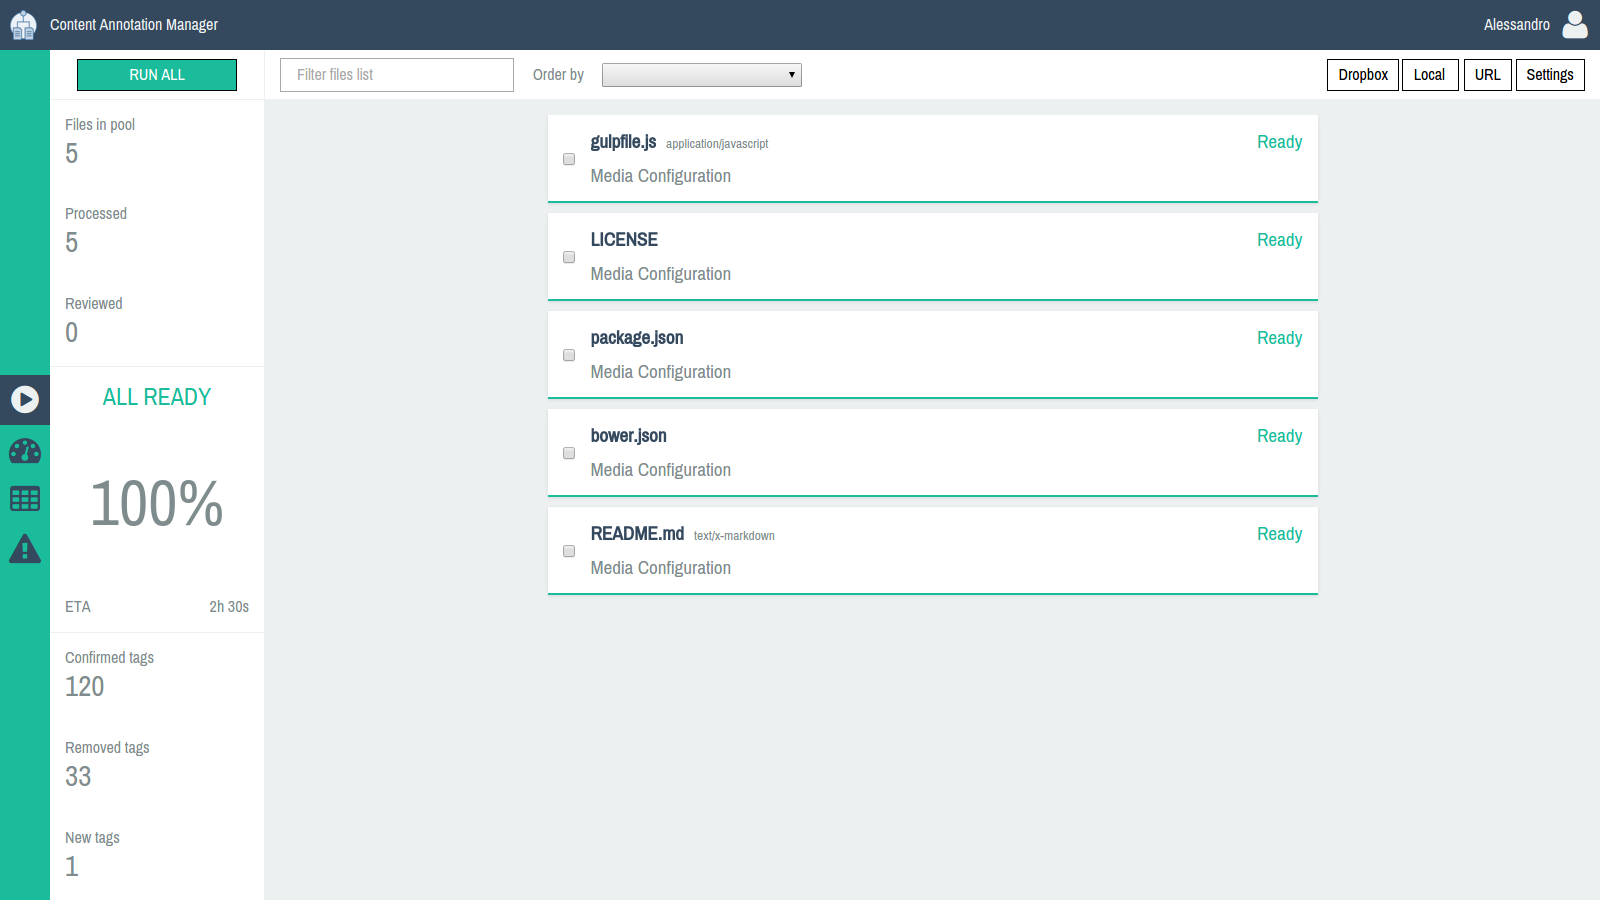
\includegraphics{./src/img/analyze-screen.png}
\caption{Analyze screen, global glance}
\end{figure}

The main content, visually representing the resource selection section.
Here, the most prominent element is the list of selected documents to be
indexed; indeed, I decided to represent each resource with a single,
well-defined, block, rather than with a simple entry in a table or list.

This is meant to be a visual signal that every single one of those
reveals a big process, involving the content augmentation job performed
by the underlying system, the tags review and modification by the human
agent, while requiring special attention in the configuration and
parameters selection, since every workflow (as it is called in CAM)
relates to a specific type of content, to some types of file (if the
document is contained in a file, as it often happens with CAM), and it
has been configured by carefully choosing the plugins to be activated
during the analysis (which, for instance, affect the way relevancy
scores are computed). Therefore, every document is spaced-out from the
others, has its own status indicator (not processed, ready, reviewed)
and its own configuration.

In this section of the application, there is a lot going on. Thus, my
approach consists in hiding as much complexity as possible by providing
a single point of contact between client and server. Indeed, the main
object the user interacts with is a ``pool'' of documents to be sent to
the server; she can populate such a pool in different ways: adding files
from a pre-configured Dropbox folder or the local hard drive, by
pointing to web resources through URLs, or even by manually entering
text (this functionality hasn't been developed yet, but it will be).
There are many things the user can do, a part from populating the pool,
such as setting different workflows to different documents, running or
re-running only some of the resources, filtering the list, changing the
parameters characterizing the workflows themselves (e.g.~which
taxonomies to use), and so on, but, by putting the list of ``to-dos''
that will be sent to server at the center, not only the user doesn't get
overwhelmed by the variety of options and nuances, but - most
importantly - she is always under control.

\chapter{Focusing on the user: from useful to
usable}\label{focusing-on-the-user-from-useful-to-usable}

Even though the technology involved is powerful and capable of really
interesting things, when designing a User Interface, the main goal
should always be focusing on the user, finding in the realization of
such design that sweet spot between extremely simple and usable and very
effective and useful. Achieving the result is not always immediate and
easy, and consists in a process of constantly putting the user at the
center. In the following, it is explained how I reasoned about this in
the most important page of the application, plus some considerations on
how animations can improve the overall UX.

\section{A UCD-based approach: the Review
screen}\label{a-ucd-based-approach-the-review-screen}

There are a couple of aspects of the review screen that certainly
demonstrate how designing for the user, or User Centered Design (UCD),
is a great approach to make more usable products. In fact, some small
additions and modification to the global behavior of CAM are entirely
due to this way of working, like the ``reset filters'' button already
mentioned, which enhances the user experience by reducing the number of
clicks to switch from one filter to the other by a great deal, adopting
a single color to highlight the terms in the text instead of using a
color per class or category, which greatly improves the readability of
the text, or providing affordances for the user to undo an action or
rollback to a previous state, for example when she deletes some tags.

\begin{figure}[htbp]
\centering

\includegraphics{./src/img/review-notification.png}
\caption{Review screen, removing notification, with possibility to undo}
\end{figure}

The greatest challenge I am facing designing the new version of CAM is
being able of both improving the existing demo and suggest new features
to be integrated in the application, so that it could be used as a
stand-alone tool in the future. While doing this, I had the chance to
modify some aspects of the user's flow, revisiting the experience. A
good example of this is the ``add tag'' action, which used to consist in
the steps:

\begin{itemize}
\itemsep1pt\parskip0pt\parsep0pt
\item
  select Class
\item
  select Label among the ones corresponding to the selected class
\end{itemize}

This probably makes a lot of sense to a developer who also knows how the
taxonomy works, but it doesn't tell much to a human indexer who usually
isn't trained in those terms. What actually happens during the usage of
this function is:

\begin{itemize}
\itemsep1pt\parskip0pt\parsep0pt
\item
  the user thinks of a tag she wants to add
\item
  the user tries to help taxonomists by indicating a class
\end{itemize}

I made the process more user friendly, by guiding through the tag
addition with a wizard, giving also the possibility not to suggest any
class, since one could not know what to do with the tag she is thinking
of. Also, I got rid of the notion of ``class'' by using the ``type''
term, which can be less confusing for some users. In addition to this, I
improved the way new tags get integrated in the UI, by adding a ``manual
entry'' type, that can be reached through the filters. As a result, the
user has a quick method to revisit what she added, and possibly change
her mind.

At this point, the ``review'' screen was still lacking a couple of
fundamental features: a way to submit the modifications and store them
on the server, and the possibility to find a tag in the document and
easily see its details in the table. A usability problem that I spotted
in the old version of CAM was the complete lack of a system to undo just
executed actions or rollback past decisions (in other words, to change
one's mind). For instance, when the user deletes a tag, it simply
disappears from the application and there's no way to restore it; or if
she adds a couple, they get lost in the midst of the possibly very long
list of tags. Finally, by hitting a ``done'' button, the user would
cause an automatic process of storing the modifications, no way back. By
analyzing such a situation, I immediately thought of an useful parallel
with the shopping carts in e-shopping websites: when you go on
Amazon.com, there is no way you can accidently end up buying something
you didn't want, nor it happens that you leave an item out of your
order. This is mostly due to the last step of the purchasing process,
represented by the shopping cart, which summarizes all the details, the
items you are about to shop, prices, and so on; in addition, there's
some confirmation action required in order to proceed further with the
order. The way I see CAM is greatly linked to this scenario: CAM's users
decide among a catalogue of tags which ones they want, which ones the
would discard, and they can even ``buy'' some tags that are not present
in the catalogue itself. Therefore, my suggestion is to add a simple
``summary'' step, in which the users are presented with a list of the
modifications that are about to be permanently stored, with the option
to roll back and change their minds.

\begin{figure}[htbp]
\centering
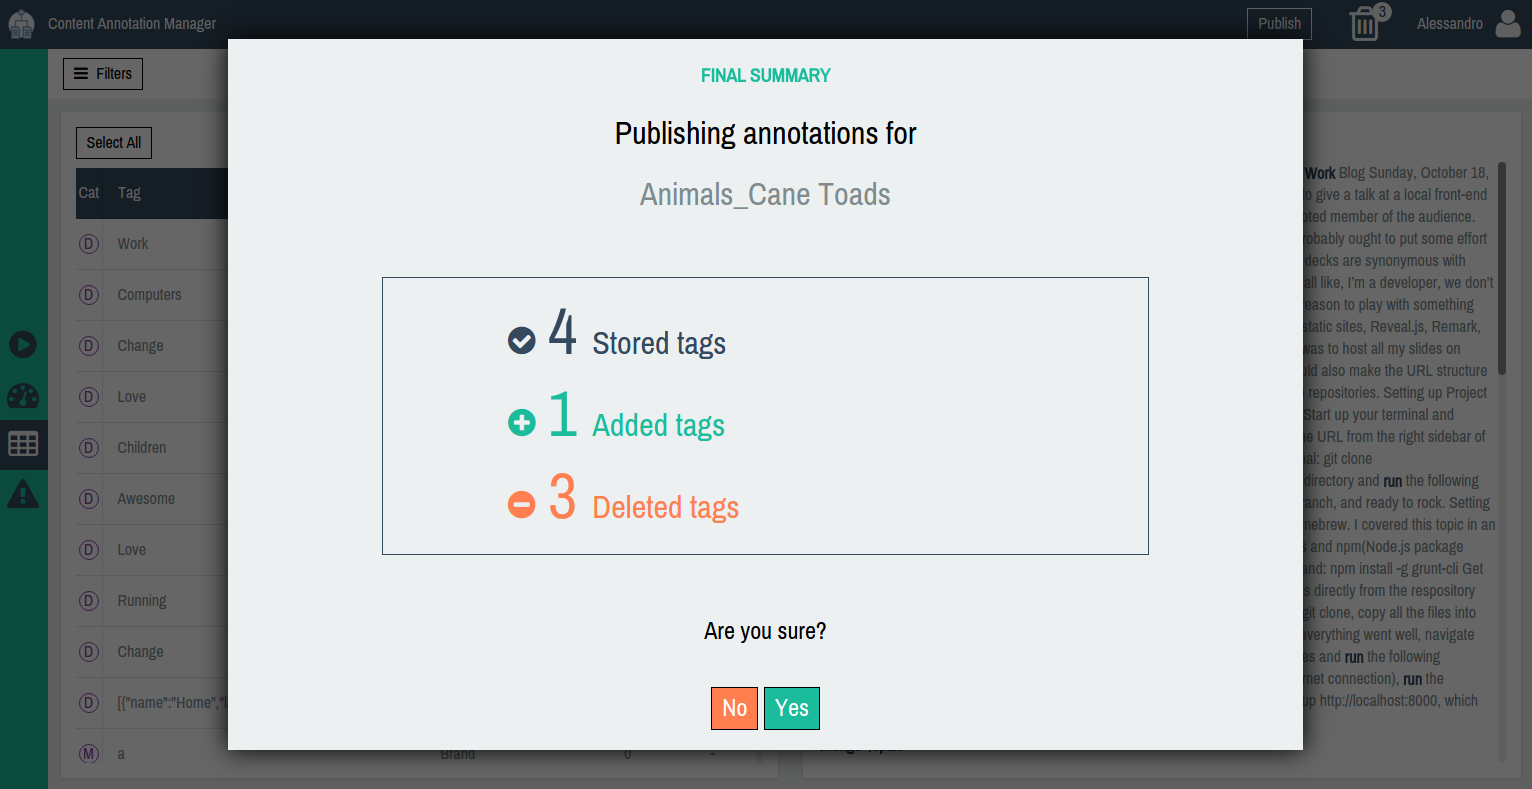
\includegraphics{./src/img/review-summary.png}
\caption{Review screen, summary}
\end{figure}

Another idea that came up aiming at supporting usability of the
application is allowing a ``right-to-left'' interaction, meaning:
instead of browsing the resources from left-to-right, starting from the
filters, then reading the table, and finally finding the interesting
tags in the document, the user might want to be able to quickly spot a
tag in the document, and then easily find the tag in the table, without
having to scroll a possibly very long list of those. The interaction to
be realized is simple: clicking on the highlighted tag in the document
should somehow cause a further filtering in the table on the left.

\section{User Experience: Animation as a
tool}\label{user-experience-animation-as-a-tool}

Contrary to what one may be tempted to believe, animation is not only a
way to make things prettier in an interface, but rather it can be a
powerful tool in the hands of a good designer: indeed, by making good
use of motion techniques and by paying attention on not falling in the
trap of cluttering the screen with too many moving elements, it is
possible to greatly enhance the usability of a product. As humans, when
we interact with some piece of software, we tend to assume that it will
behave as real things do in the real word. The term behaviour is pretty
powerful, but it helps conveying the message that we implicitly think of
shapes and UI components as real things, and as such, we expect them to
follow the same basic principles:

\begin{itemize}
\itemsep1pt\parskip0pt\parsep0pt
\item
  objects accelerate and decelerate, rather than abruptly stopping when
  they have reached their destination
\item
  objects don't enter in and exit from sight ``teleporting'' themselves
  into view
\end{itemize}

When this implicit pact is broken by a UI element, two things happen in
one's mind:

\begin{itemize}
\itemsep1pt\parskip0pt\parsep0pt
\item
  first, the user needs to realize that something happened; for
  instance, a dropdown menu changing from collapsed state to expanded
  state
\item
  then, the user's brain needs to figure out what happened; in this
  example, it needs to reconstruct all the missing `frames', in order to
  figure out the change of state
\end{itemize}

This process is really fast, but it has the negative effect of
interrupting the user's flow and, therefore, it affects the overall
experience. Thus, keeping in mind these principles, I played with
animations and implemented smooth state changes, with the goal of easing
the user's way through the application; indeed, since animated
transitions can work as intermediaries between different UI states and
can help orientate users, I focused on two major state changes in the
``review'' screen and studied how I could put all these notions together
and help the user understanding not only the sequence of events, but
also sorting out causes and effects. In the ``review'' screen, there is
the main content, as usual, and some additional filters to act on in a
sidebar. This bar isn't always needed, so it makes sense to hide it
behind a button and to show it only when the user really wants to
interact with it; however, when visible, it doesn't overlap the rest of
the content, but rather it pushes it on the right, causing a big change
in all the elements the user just got used to seeing. In presence of big
state changes like this, it is important that the UI doesn't surprise
the user in a negative way, by moving things on the screen without her
understanding where they went, or where they came from. I thus decided
to animate the scene, so that the user can follow the motion of an
element to understand how the before state of the page and the after
state relate to each other.

\begin{figure}[htbp]
\centering
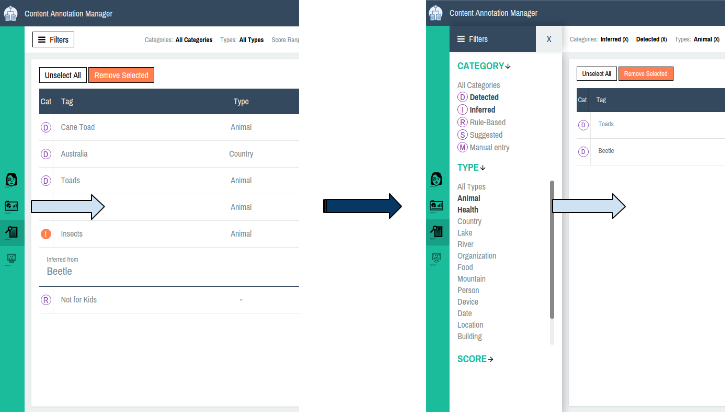
\includegraphics{./src/img/review-sidebar-animation.png}
\caption{Review screen, sidebar animation}
\end{figure}

Another abrupt change that I wanted to avoid is the elimination of a
tag. When a tag is deleted from the table, it disappears and can be
found, and possibly restored, by clicking on the bin icon on the
upper-right corner of the application. This is a perfect example of how
a simple animation can solve a big usability issue, since it takes a
huge mental leap in order to understand that an entry in the table just
got transferred to another place of the application, without having to
remember where things go when they get deleted. Also, this problem shows
how true it is that we always expect UI's objects to behave as normal
things in the real word: when you throw away something, it doesn't
materialize itself in the trash bin, then it shouldn't be happening in
the virtual world. So how can an animation solve this issue? Nothing too
fancy, but a simple notification-style popup that slides in from the
right in the upper-right corner of the screen, accomplishing two tasks
at once: on one hand, it gives the user the possibility to undo the
action, while on the other hand, it suggests, or reminds, where the tag
has just gone to, by sliding up towards the bin icon when disappearing.

\begin{figure}[htbp]
\centering
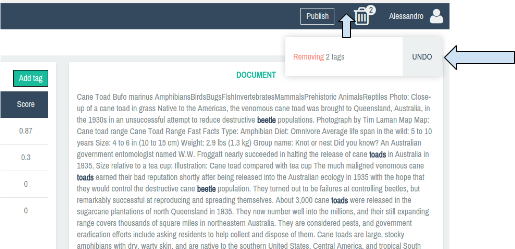
\includegraphics{./src/img/review-notification-animation.png}
\caption{Review screen, notification animation}
\end{figure}

\chapter{Perfmatters: a deep dive into
performance}\label{perfmatters-a-deep-dive-into-performance}

When it comes to performance on the web, more and more often developers
don't take into account the external factors that constrain an
application's speed, which don't depend on architectural patterns or
optimized data structures. However, those are the real bottlenecks in
the web of today, especially when targeting a desktop environment, where
developers can count on medium to high processing power. I believe this
is a really important problem to address for CAM, and other Mondeca's
products as well, since we are not producing applications to be used on
mobile; in addition, most of the jobs and features that such products
offer are run on servers, therefore the client needs to continuously
rely on network requests and gets slowed down by the decently big amount
of data that needs to be transferred on the wire. For these reasons, it
feels compelling to reduce the impact on performance of elements that
are independent from the execution of the jobs themselves. Most
commonly, such elements are the following:

\begin{itemize}
\itemsep1pt\parskip0pt\parsep0pt
\item
  \emph{file size}, which basically determines the amount of time spent
  by the browser on downloading the assets needed to display the
  requested resource; this can be greatly reduced by means of
  established techniques such as minification and compression of assets
\item
  \emph{number of HTTP requests}, which greatly affects the bootstrap of
  a web page since every HTTP connection that the client needs to open
  adds a fairly significant overhead, which is generally big compared to
  the time the client will actually spend downloading the resource,
  especially when such a resource has been minified and compressed; it
  exists a simple and powerful solution to this problems, which consists
  in concatenating as many resources as possible in a single file. This
  technique, when combined with the previous ones that aim at reducing
  the file size, can optimize the loading time by a great factor
\end{itemize}

By means of concatenation, minification and compression techniques, the
page can load faster and feel instantaneous to the user. However, other
things can be done in order to further improve the experience for the
user; first of all, though, it's important to have valid measurements in
order to understand what needs to be improved, take action and then
validate the results. Thus, I performed a performance audit on CAM,
tested some solutions and then evaluated the effects against some known
indexes and thresholds.

\section{Two metrics: loading speed}\label{two-metrics-loading-speed}

As the current state of the application is at its earliest stages, I
mainly focused on two ``metrics'' for performance gage: loading speed
and runtime smoothness. Please also note that, at the time these
measurements were taken, no actual server-side processing was taking
place, and the actual data shown by the application was mocked-up and
dished out as a JSON file to the requesting client. Even though this may
seem to be invalidating the measurements, being that I am referring to a
situation that it's not going to be replicated in real use case
scenarios, it is actually meaningful to try and optimize the performance
of the application at this point in time, since my goal, as a front-end
developer, is to reduce the impact of the application shell on the
global performance as much as possible, possibly shooting at adding an
overhead to the whole process of indexing documents that can be
considered as negligible.

Let's start with loading speed. The most common metric referred to when
assessing loading speed is the so called speed index, which basically is
the average time at which visible parts of the page are displayed,
expressed in milliseconds. As the \emph{webpagetest.org} documentation
puts it (emphasis added)

\begin{quotationb}
``The Speed Index metric was added to WebPagetest in April, 2012 and
measures \textbf{how quickly the page contents are visually populated}
(where lower numbers are better). It is particularly useful for
comparing experiences of pages against each other (before/after
optimizing, my site vs competitor, etc) and should be used in
combination with the other metrics (load time, start render, etc) to
better understand a site's performance.''
\end{quotationb}

Webpagetest.org is one of the most popular and useful online tools for
performance evaluation on the web; it basically runs a tests suite over
a given URL and outputs a series of tips to improve the performance and
important measures to be aware of. For the sake of this first
experiment, I am only reporting the Speed Index, which was
\textbf{4575}. This figure doesn't tell a lot per se, but it is
important to know that a solid speed index value is around 1000, as it
will be covered in the next sections.

In order to dig deeper into what could be causing a lower loading speed
than expected, I took a look at both the network usage and the
JavaScript profile, thanks to the Chrome DevTools. The network traffic
analysis revealed that the client was spending too much time downloading
the resources, and this was slowing down the first paint of the page;
thus, the first improvement I made was relying on the established
techniques explained in the previous paragraphs: indeed, by means of
concatenation, minification and compression techniques the time to first
paint dropped down from roughly 1 second to 0.5 seconds, on my testing
environment. The reason why this happens lies in the way the browser's
parser is dealing with external resources when first analyzing (and then
rendering) a page: it goes from top to bottom through the HTML file, it
fetches the resource from the server every time it encounters a script
tag or style link, and only then, the first paint appearing on screen
can take place. It needs to be acknowledged that the speed index is
taking into account the time at which the page is \textbf{mostly
visually complete}, whereas the time to first paint it's just the moment
at which the browser can actually \textbf{start rendering} pixels on the
screen. There is an important difference between the two metrics, which
can be brought down to a single fundamental concept: perceived
performance.

\section{An orthogonal metric: perceived
performance}\label{an-orthogonal-metric-perceived-performance}

At the same way UCD predicates designing for the user, we shall put the
user at the center while improving performance. Opposed to computational
performance, perceived performance refers to how quickly a process
appears to be completed to the user, which may often differ from the
actual speed that process has been completed at. For instance, the
amount of time an application takes to start up, or a file to download,
is not made any faster by showing a splash screen or a progress bar.
However, it satisfies some human needs: it appears faster to the user as
well as providing a visual cue to let them know the system is handling
their request. This is a very relied upon technique when trying to
deliver a great experience of use for a not-so-snappy system; when it
comes to web applications, the goal is to be able to display parts or
previews of the final status the screen will reach, while loading it.
Therefore, coming back to difference between speed index and time to
first paint, the latter doesn't give an accurate indication of how
responsive the application will be \textbf{perceived}. In this context,
recently it has been gaining a lot of popularity a new technique
consisting in showing the application shell as quickly as possible, then
dynamically injecting content into the page. In order to achieve this, I
had to first solve another issue that was heavily affecting the pages
load time, causing that 4000+ speed index to be so high; that is, an
Angular project is typically composed of a lot of HTML templates, in
order to enhance code readability and maintainability. However, the
downside of such a module-based approach, is that every directive or
template included in the page is going to trigger an HTTP GET to the
server requesting for the corresponding HTML file. So how do we solve
this problem? I tested three solutions, basically building every new
idea on top of the previous one.

At first, I enabled templates \textbf{caching} through use of Angular's
\texttt{\$templateCache} service. This allows Angular to fetch every
template only once, and reuse it throughout the whole application every
time it is requested again. While such a strategy improves the overall
navigation experience, it still doesn't solve the problem of having to
contact the server the first time an asset is needed. Then, I instructed
the application to \textbf{prefetch} all the HTML assets after all the
core requests have been handled and the first page has been completely
loaded. The objective of such a strategy is to prepare the cache with
all the assets that will be needed in other sections or pages, even they
may be hidden at first. While this two improvements, when applied
together, greatly reduce the delays introduced by the need of
continuously fetching the HTML templates, they don't improve the
perceived speed of the application, rather they deal with the
computational one. The user was still looking at a blank page until all
the resources were ready: indeed, such caching and prefetching
strategies rely on Angular to be fully loaded and functioning.
Therefore, I decided to \textbf{inline} all the templates into a single,
minified, JavaScript file (under the form of simple strings) and to
include such a resource into the index.html. But why is this any better
than the previous solutions? Here's what happens in the browser in the
two situations:

Without inlining:

\begin{itemize}
\itemsep1pt\parskip0pt\parsep0pt
\item
  the browser fetches the index.html
\item
  the browser fetches the script.min.js, which is the file containing
  all the application's code
\item
  the browser runs such script, which will then fetch the missing
  templates from the server
\item
  while the network request is still pending, the browser goes on
  parsing and rendering the first page, asking \textbf{to the server}
  every HTML template it needs for the first load
\end{itemize}

With inlining:

\begin{itemize}
\itemsep1pt\parskip0pt\parsep0pt
\item
  the browser fetches the index.html
\item
  the browser fetches the script.min.js
\item
  the browser fetches a brand new templates.min.js file, containing
  inline declarations of all the templates used throughout the
  application
\item
  the browser goes on parsing and rendering the first page, asking
  \textbf{to the cache} every HTML template it needs for the first load
\end{itemize}

Even though the difference may not seem that big, it has great
implications on the perceived loading speed. Indeed, the user is now
almost immediately shown the application shell, meaning that the whole
structure of the application (header, navigation bar, sidebar, and so
on) is almost immediately rendered, while the dynamically injected
content gets displayed as soon as it is available. However, in order to
better define the viability of this approach, one must define what
``almost immediately'' means, and understand why adding one HTTP request
at the beginning of the page loading process (that template.min.js
additional resource) feels faster to the user, than it does fetching an
HTML template when needed. The ``application shell'' strategy is backed
up by several studies, and has its roots in the publication
\emph{Response Times: The 3 Important Limits} by Jakob Nielsen on
January 1, 1993. Thanks to this study, we can now quantify qualitative
measurements such as ``immediate'' and ``instantaneous'': indeed,
Nielsen proved that a waiting time under 100ms feels instantaneous,
while a waiting time around 1000ms signifies a context switch to the
user. Further analysis have further expanded these concepts and, most
recently, have led to the definition of the RAIL model, which is defined
as by the Chrome team who came up with this new concept as (emphasis
mine):

\begin{quotationb}
``a \textbf{user-centric performance model}. Every web app has these
four distinct aspects to its life cycle, and performance fits into them
in very different ways: Response, Animation, Idle and Load''
\end{quotationb}

Basically, the RAIL model gives us developers a few figures that we can
refer to whenever we are facing challenges in improving the perceived
performance; indeed, thanks to RAIL, we are finally left with the
following timing constraints:

\begin{itemize}
\itemsep1pt\parskip0pt\parsep0pt
\item
  16ms per frame during an animation
\item
  100ms of response time, upon user's interaction
\item
  1000ms of loading time
\end{itemize}

But let's bring this back to CAM. This model explains why the inlining
strategy is so successful: during load time, we're working with a 1000ms
time span, during which the browser can fetch the additional
templates.min.js file. It's perfectly fine for the user to be waiting up
to 1 second for the application to load, thus one can make use of this
and load the templates resource; as a consequence, two milestones are
achieved:

\begin{itemize}
\itemsep1pt\parskip0pt\parsep0pt
\item
  the user sees the application shell all at once, in under a second
  time, and mentally establishes that the loading phase is done (even if
  it's not);
\item
  when the user will change views or pages, all the structural element
  will be immediately in place, giving the perception of instantaneous
  navigation
\end{itemize}

Here's what the pages look like before the content is dynamically
injected.

\begin{figure}[htbp]
\centering
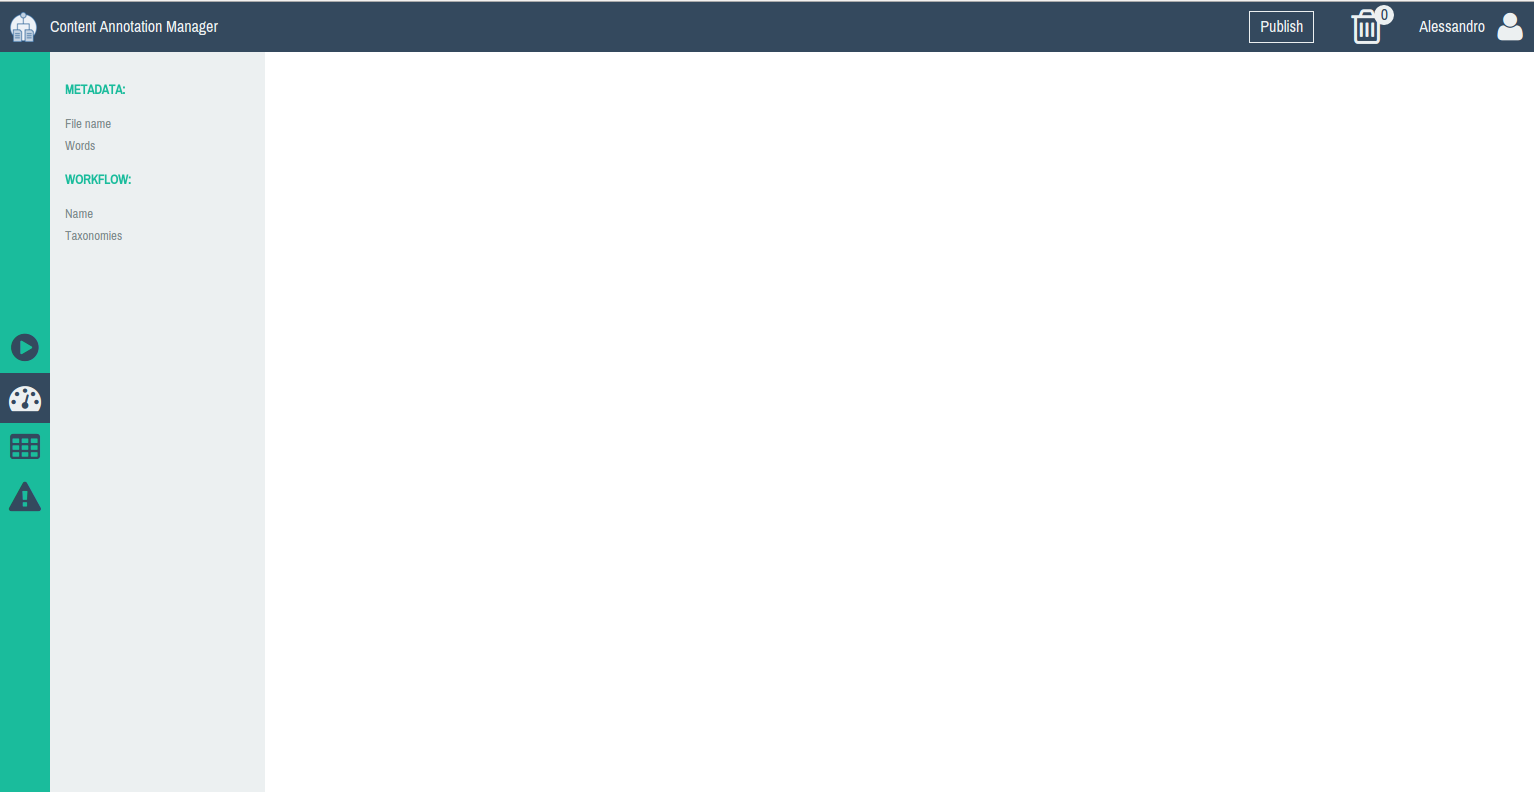
\includegraphics{./src/img/overview-appshell.png}
\caption{Overview screen, application shell}
\end{figure}

\begin{figure}[htbp]
\centering
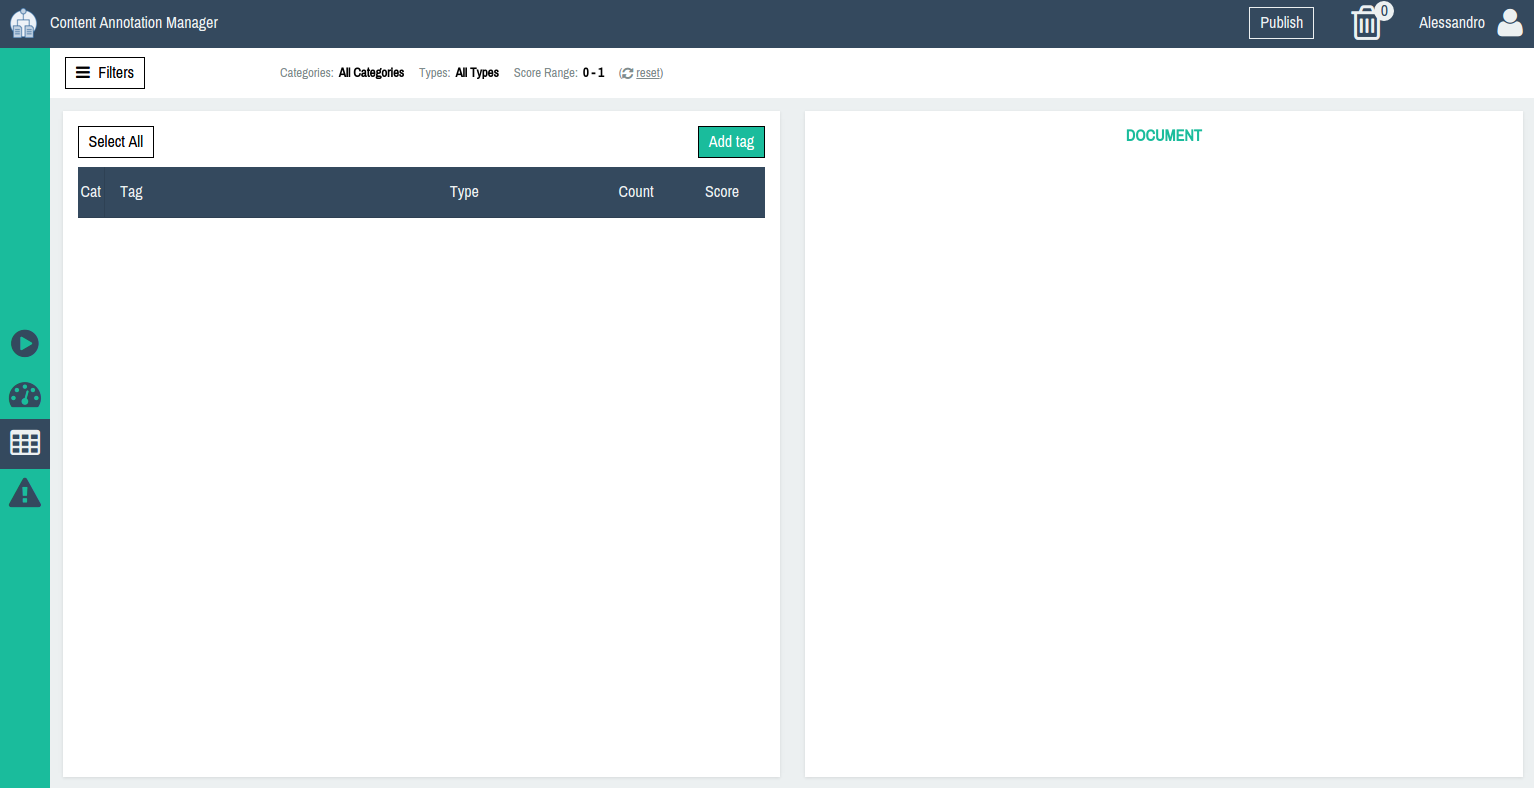
\includegraphics{./src/img/review-appshell.png}
\caption{Review screen, application shell}
\end{figure}

\section{Two metrics: runtime
smoothness}\label{two-metrics-runtime-smoothness}

Regarding the runtime smoothness of the application, a few tweaks needed
to be done. First of all, the meaningful metric here is the frames per
seconds (FPS), the goal is to ensure that animations and scrolling play
out at 60fps, and again I relied on the Chrome DevTools in order to
reliably get this information. Since the ``analyze'' screen is basically
mostly static, I focused on the ``review'' and ``overview'' screen; both
of them used to have some performance issues in terms of animation
smoothness, but the origin of such low fps turned out to be very
different in the two cases. In the ``overview'' screen, a visible lag
could be seen while first loading the page, and this feeling was
confirmed by the depressing value of 3fps in some steps; indeed, the
charts are animated (bars grow to their final size, pies build up in a
fancy way) as soon as the page is loaded. A deep look into the Timeline
view in the tools revealed what was causing it: the Angular's directive
I am using to stamp out those charts (which is basically wrapping the
Highcharts.js API) was running its underlying JavaScript in order to
make the animation happen. Regardless of whether or not this might be
the right way to do it (more often than not, such JavaScript-empowered
transitions do not rely on GPU acceleration, even though I can't be sure
since I didn't dig into the implementation code of it), this was causing
the browser to spend a lot of time on every single frame, while, since
we are aiming to rendering at 60fps, we are left with less than 16ms per
frame; moreover, by further analyzing the timeline, we can see 8
``spikes'', which bring to the surface another problem: the directives
are running too many times, in fact one can see 8 ``charts'' loading and
drawing, while only 4 are being display on screen. Why is this
happening?

\begin{figure}[htbp]
\centering
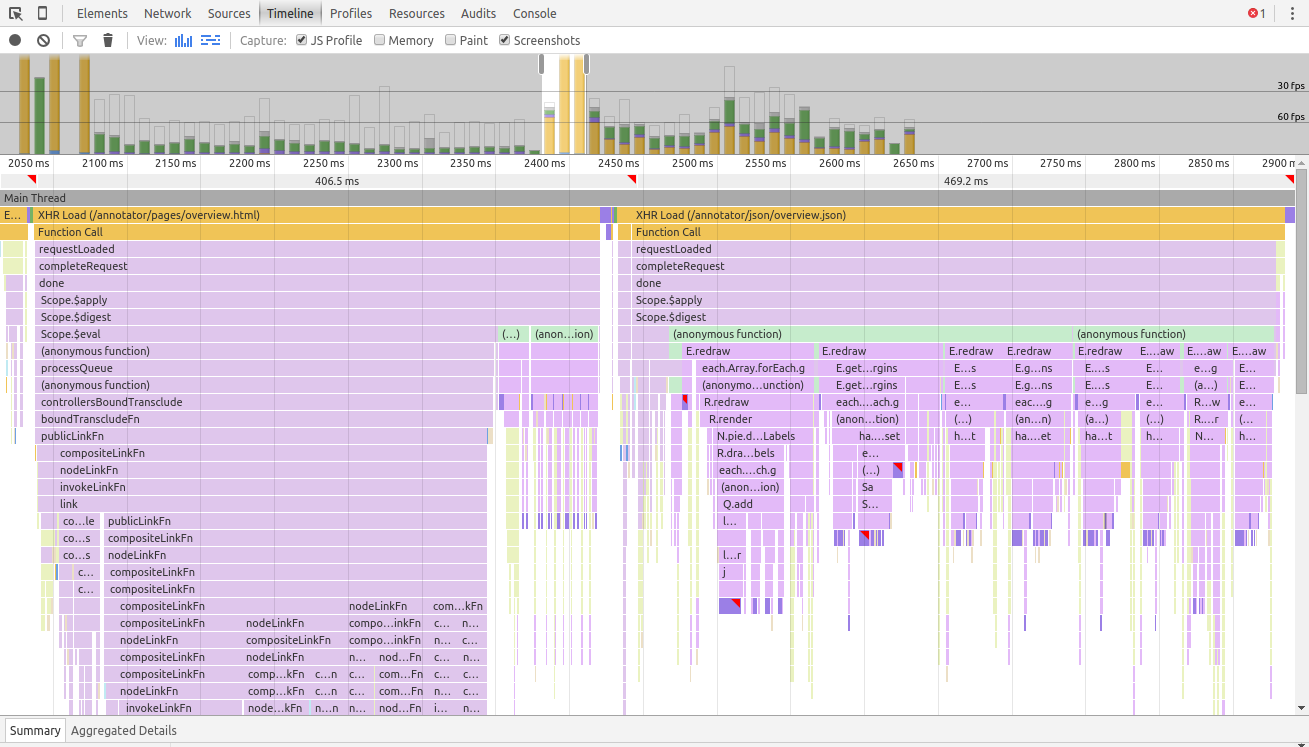
\includegraphics{./src/img/overview-jsprofile.png}
\caption{Overview screen, JavaScript profile in the Timeline}
\end{figure}

This page was built with two versions in mind, one that should be
displayed when the cluster-based scoring plugin is available, and one
when it's not. In order to achieve this effect without duplicating too
much code, I was simply hiding and showing widgets as needed,
programmatically. However, for how Angular's directives work, the
hiding/showing action takes place after the basic directive
functionalities are loaded (needed DOM is linked to the root element,
controller's code has run, and so on). Therefore, exploiting the fact
that every HTML template I'd need is going to be precached at load time
anyway, I decided to split such a page into its two versions; by doing
this, I solved the performance issue, while making the code much more
readable and maintainable. It's also worth noting that in Angular it can
be possible to lazy load the directives, which would have solved the
issue as well, but I decided nonetheless to take the ``maintainability
path''.

Much a different process was fixing the performance issues in the review
screen. While the previous one had a lot to do with the JavaScript being
run, this one finds its causes in the way CSS properties are
transitioned by the browser's rendering engine. First of all, a little
bit of context: in the review screen, the transition between filters bar
closed and filters bar open states is animated, provoking the subsequent
reduction of both the width and the font-size of the tags' table and
document container. As it turns out, this can be cumbersome to render at
60fps with the current technologies, for the way the engine takes care
of those properties change; for the sake of this report, what matters is
that maximum performance can be obtained only when tinkering with
transform and opacity, which, as it currently stands, are the only
properties that don't trigger neither the layout nor the painting steps
of the rendering process.

\begin{figure}[htbp]
\centering
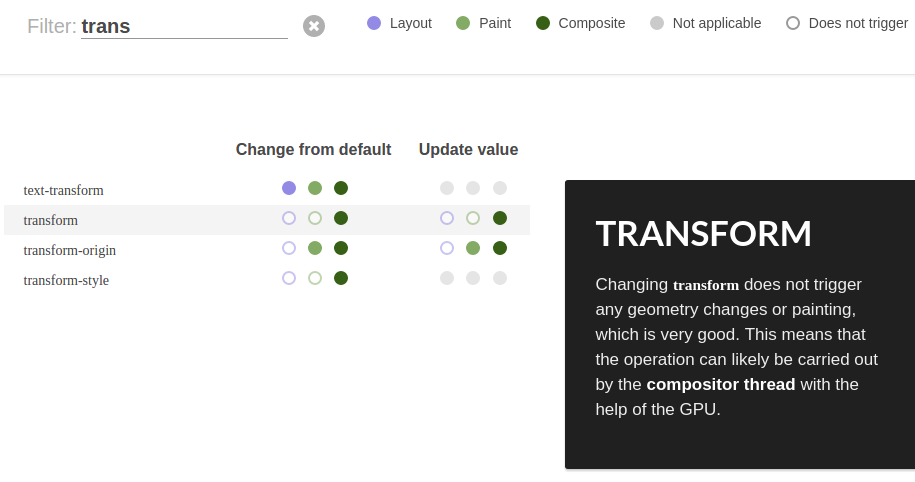
\includegraphics{./src/img/csstriggers.png}
\caption{http://csstriggers.com/ - It offers a quick summary of which
CSS properties trigger which phase of the rendering process}
\end{figure}

Therefore, one might think that the fix would simply consist in
animating the transform property of the filters, in order to exploit GPU
acceleration; however, this was already the case, as the filters' box
was translating into view by means of transform: \texttt{translateX(0)}.
What was missing was a hint to the browser, telling it that the HTML
element containing the filters' box was going to change its transform
property, thus allowing it to be layer-promoted. Without going too much
into the technicalities of this procedure, whenever a moving element
needs to be computed by the compositor thread, it also needs to live
within its own layer; in the past, in order to place an element inside a
new layer, there was the need to use the transform:
\texttt{translateZ(0)} hack, which was basically forcing
layer-promotion. Today however, it suffices to use will-change:
transform, which enables every kind of optimization for that kind of
transition by the rendering engine, layer-promotion included.

\chapter{The back-end: architecture, new features and the legacy
problem}\label{the-back-end-architecture-new-features-and-the-legacy-problem}

During my fifth month as intern, I worked on the back-end side of the
project, my tasks being refactoring the existing code, developing new
features and integrating it on the front-end.

\section{Architecture}\label{architecture}

As I step in and take charge of the back-end of the web application for
CAM, a valuable and rich code base already exists. Let's quickly review
the architecture of the system, by listing its components.

\begin{figure}[htbp]
\centering
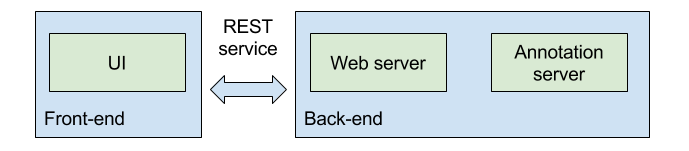
\includegraphics{./src/img/architecture.png}
\caption{CAM Architecture}
\end{figure}

On the front-end, the UI we discussed so far. On the back-end instead,
there exist two separate and independent components:

\begin{itemize}
\itemsep1pt\parskip0pt\parsep0pt
\item
  the \emph{Annotation server}, it's the core engine of the whole CAM
  system. It's capable of analyzing, mining and augmenting the documents
  in input, and it outputs in RDF/XML format
\item
  the \emph{Web Server}, which acts as mediator between the client and
  the Annotation server, has two primary roles: serving static and
  dynamic assets to the client, and fetching live analysis data from the
  Annotation server
\end{itemize}

Since a basic UI for CAM already existed in the past, a Web server is
already set up and most of the work needed to parse the RDF results and
build an Object representation of it in memory is already available, and
therefore there's no necessity to rebuild everything from scratch. The
problem however is that the new client application is expecting certain
input data - some of them totally new - with a given structure, in a
JSON format, and so on. My job then is to re-factor the existing data
into a more suitable shape, develop and build new features and
aggregations on top of the available ones, and integrate such a suite of
services on the client, by means of a simple RESTful type of service. I
thus decided to create a \emph{mediator} module, sitting between client
and server, capable of managing the interactions between the two through
an API, which exposes the minimal interface needed to make it work; by
doing this, I decouple as much as possible both the UI and the already
existing Web server, allowing future versions of either one of the other
to be easily plugged in or replaced. In addition to this, my module
abstracts the interactions and hides as much as possible the underlying
processing jobs that take place on the web server, aiming to support
Mondeca's decision to outsource CAM's UI maintenance to another company
in the future.

\section{Module's structure}\label{modules-structure}

The new module exposes the following services:

\begin{itemize}
\itemsep1pt\parskip0pt\parsep0pt
\item
  \texttt{getAnalyzeData}, which returns all data needed by the Analyze
  page
\item
  \texttt{getOverviewData}, \texttt{getReviewData} and
  \texttt{getTroubleshootingData}, which take a document and return the
  relative data
\item
  \texttt{indexDocument}, which takes a document and perform the right
  analysis, depending on the document's type (is it URL, free text,
  binary data, and so on)
\item
  \texttt{getProgress}, which returns the current progress of the
  analysis process
\item
  \texttt{publish}, which takes all user's modifications made to the
  analysis results, and stores them
\end{itemize}

This reduces by a big amount the total surface of the API, which used to
be bigger and, therefore, much less maintainable and too tightly coupled
to the client's implementation. On the other hand, by using less finely
grained services there exist the risk of making it too difficult to
split pages on the client in smaller pages. This is a trade-off between
ergonomics and adaptability, however I prefer this approach since it
allows new developers to easily get on board and start writing code from
their first day on both the client and server, without having too much
to learn about client-server interactions; in addition to this, offering
few and ``big'' services encourage front-end programmers to fetch all
the needed data in one single request at load time, which, as described
in Chapter 5, can be a big win in terms of both perceived and
computational performance. Even though the basic structure of the module
might seem completely RESTful, there are a couple of exceptions:

\begin{itemize}
\itemsep1pt\parskip0pt\parsep0pt
\item
  the \texttt{login} service, which makes use of cookies to authenticate
  the user in the following requests; this isn't completely RESTless,
  since it doesn't make use of such cookies to store session data
\item
  the \texttt{getProgress} service, which, at every call, exposes some
  session-tied state the server is keeping (the progress of the analysis
  asked by the user)
\end{itemize}

\section{Data refactoring}\label{data-refactoring}

As mentioned in the previous paragraphs, one of the main goals of the
mediator module is to re-factor the result into a more suitable format,
while enriching it by pre-computing useful aggregation such as totals,
counts, and so on. In other words, starting from a list of tags, I moved
the complexity on the server by preparing all the statistics needed in
the Overview page, collecting the list the Dropbox files in the
configured folder for the Analyze data (anticipating the eventual
request), and so on. In addition to this, the module enriches the output
of the analysis by flagging the annotations basing on their category (is
a given tag an inference or has it been extracted from the text?). The
whole process might seem a small addition to the global picture, however
it is of the uttermost importance that the Web Server undertakes the
task of preparing all the data the client might need, supporting as many
activities, aggregations and flexibility as possible, and this stands
true especially if one thinks of the API as an abstraction layer,
enabling client applications that are insightful and performant.

\section{New features and legacy's
improvement}\label{new-features-and-legacys-improvement}

Because the new \emph{CamAPI} I introduce sits in between client and
server, I had the possibility to rethink the way the two endpoint
interact with each other, focusing on improving both performance and
user experience; even though the legacy code plays the biggest part of
the back-end implementation, there are plenty of opportunities to
enhance the existent. Therefore, I contributed with four new features:
asynchronous indexation, parallelization, results caching and progress
tracking.

\subsubsection*{Asynchronous indexation}\label{asynchronous-indexation}
\addcontentsline{toc}{subsubsection}{Asynchronous indexation}

In the old CAM, while a document is being processed, the client waits
for the process to be finished and gets the result back as soon as it
completes in a synchronous fashion. There are two severe drawbacks of
this approach: on one side, the client is forced to process one resource
at a time, on the other side, the full result of the analysis needs to
be transfered on the wire, which may be fairly big and caused in the
past several problems for the too heavy payload. My solution for this
issue is to break the interaction into smaller pieces and make the
exchange of information between client and server asynchronous, as
follows:

\begin{itemize}
\itemsep1pt\parskip0pt\parsep0pt
\item
  client initiates indexation process of a document
\item
  server processes the result
\item
  client is free to ask for the result as soon as it needs it
\end{itemize}

Such an approach is not only more suitable for an user interface (which
usually implies a lot of asynchronous operations), but opens up to new
opportunities.

\subsubsection*{Parallelization}\label{parallelization}
\addcontentsline{toc}{subsubsection}{Parallelization}

The most important enhancement made possible by the asynchronism of the
requests is the capability for the client to trigger more than one
analysis at once, in a parallel fashion. In my new design, indeed, a
``pool'' of documents is created and it is then sent to the server for
analysis. The advantage is evident: there is now a much higher
throughput of processed documents. From an implementation point of view,
one could have done better than I did; in fact, in order to process more
than one document at the same time, I simply open more than one
connection to the server (the number of which is, in most browsers,
limited to 6). The web server handles every incoming request with a
separate thread, thus true parallelism is achieved. However, a much
smarter solution would have been sending the list of documents to the
server (the so called \emph{pool}), and have it creating threads; in
this way, more than 6 documents could be processed at a time, and just a
single network request should have been opened on the client. The reason
why I didn't take this path is for it would have taken too much time for
me to implement a thread pool on the server, and I was told not to spend
too much energy on the back-end, since the company is mostly interested
in an usable interface, rather than having me prioritizing parallel
execution of more than 6 resources. In addition to this, when the pool
contains a lot of documents, the whole system is blocked waiting for
every resource - possibly big files - to be transferred to the server,
therefore canceling the benefit of parallelism.

\subsubsection*{Results caching}\label{results-caching}
\addcontentsline{toc}{subsubsection}{Results caching}

In order to enable the client to asynchronously request for the result
of a given document's analysis, it is necessary to have a session-linked
results cache on the server; this ultimately solves the problem of
having a possibly too big payload to be served in a single connection,
since the client can now specifically ask for the parts of the result it
is interested in at that precise time: when the user is on the Overview
page, there's no need to fetch the data that would only be used in the
Review page, nor the log messages that can be accessed in the
Troubleshooting section. Since in the desktop environment CAM targets
the network is almost always the performance bottleneck, such a strategy
has the more general benefit of increasing the overall responsiveness of
the application.

\subsubsection*{Progress tracking}\label{progress-tracking}
\addcontentsline{toc}{subsubsection}{Progress tracking}

Finally, I introduce in CAM a progress bar showing the percentage of
completion of every document (which makes sense now that parallel
execution is present), plus a global progress indicator which relates to
all the resources being processed. As I proceeded submitting my plan to
the members of the team who used to work on CAM in the past, I
immediately encountered some resistance in introducing the progress
tracking; this was not because there is something wrong with the idea
itself, but it turned out there's no actual way to get such information
from the annotation server, which basically processes the whole document
in a stateless manner.

While this may seem a small detail in the entirety of the CAM
application, there are some considerations to make on the user
experience of it when no progress tracking is available. One of the most
important phase of the interaction between a person and an object (being
it a real or a virtual one) is the \textbf{feedback} the person is
presented with, indeed, without some sort of hint that the interaction
took place, we usually tend to be doubtful of the success of the
operation: \emph{did I click the button? did the system receive my
command?} While this is very true for every interaction, it is even more
fundamental when talking long activities. In the old CAM there is no way
to estimate the amount of time remaining, so the user can't take
decisions upon that: \emph{can I switch to some other task while I wait?
should I skip that resource, and work on simpler ones for the moment? Am
I to wait an hour or a minute?} Thus, I started to investigate how this
may be achieved, because I believe that a rough and imprecise indication
is much better than no indication in this case.

By digging a little bit more into the problem, I found out that, while
the annotation server does its job in a single run, the web server still
needs to post-process the result in several ways, before storing the
result. In such a multi-step way of proceeding I saw an opportunity to
achieve my goal: I identified 5 steps that measured a non-negligible
amount of time to complete and used those as an indicator of how far in
the processing of the document the system is. I am highly confident
that, even though the 5 steps don't take the same time and they are
really not much meaningful in terms of the actual activities they
correspond to, it is still a big win to be able to present to the user
of an estimation of how much work is done and how much is yet to be.

\chapter{Wrap up: i18n, future work and
conclusions}\label{wrap-up-i18n-future-work-and-conclusions}

In order to conclude the description of the CAM project, it is worth
mentioning how the application is internationalized; in addition, since
Mondeca believes in the future of such a product, some considerations on
the future work that can be done to further improve the experience are
included in this final chapter.

\section{i18n}\label{i18n}

A special effort required on my side has been internationalizing CAM in
order to enable translation of the app at two different levels: the goal
is to support multiple languages in both the UI's text and labels, and
in the underlying data; for instance, a French document can be then
reviewed with in English, meaning the labels for classes, entities and
annotations will be displayed in the selected language.

\subsection{The UI level}\label{the-ui-level}

On the UI, my approach consists in relying on a configuration file, more
precisely a JSON structure, containing all the labels that are used in
the interface; the configuration allows to plug in as many translations
as needed, under the form of additional JSON structures. From a
technical point of view, I created a \emph{Translations} module to set
up all the supported languages; in addition, the \emph{translate}
Angular's filter is used in order to enable dynamic change of language,
via a simple pop-up window. What this means is that, at any point in
time, the user can select another language and see the whole application
translated in almost no time. The benefits of the selected solution are
the possibility for a non-technical member of the company to review, and
easily change, the copywriting, or to an external translator to quickly
add a new language by simply providing the key/value pairs (e.g.
`HELLO': `Salut'), which can be very important when a company needs to
move fast and to adapt their product to the customer's needs.

\subsection{The data level}\label{the-data-level}

As already mentioned, the underlying system can be tuned to analyze
resources in different languages; in addition to this, the taxonomy can,
and usually does, contain labels in different languages: the
\emph{House} entity therefore will have a \texttt{label\_en}
\emph{House}, a \texttt{label\_fr} \emph{Maison} and a
\texttt{label\_de} \emph{Haus}, depending on the configuration. By
exploiting this information, the web application allows the user to
change the language for the data, by choosing among the available ones
advertised by the annotation server. The implementation is pretty
straightforward: the web server lists the available languages at
bootstrap time, then sends every label in multiple languages in order to
avoid having the client requesting the data twice, the UI displays data
in the selected (or default) language. Therefore, I simply introduced a
\emph{i18n} module, which handles default language, current language,
corner cases such as \emph{no language} and provides a simple
\texttt{extractName} method to be used by the views to extract the label
in the correct language from the given entity or class or else.

\section{Future work}\label{future-work}

\section{Conclusions}\label{conclusions}

\chapter*{Bibliography}\label{bibliography}
\addcontentsline{toc}{chapter}{Bibliography}


Cao, Jerry, Tom Green, and Marek Bowers. 2015. \emph{The Guide to
Interactive Wireframing}. UXPin.

Cao, Jerry, Kamil Zieba, Krzysztof Stryjewski, and Matt Ellis. 2015.
\emph{Web UI Design for the Human Eye: Colors, Space, Contrast}. UXPin.

Colborne, Giles. 2010. \emph{Simple and Usable: Web, Mobile and
Interaction Design}. New Riders.

Nielsen, Jakob. 1993. ``Response Times: the 3 Important Limits.'' In
\emph{Usability Engineering}. Morgan Kaufmann Pub.

Norman, Donald. 2013. \emph{The Design of Everyday Things: Revised and
Expanded Edition}. Basic Books.

Soegaard, Mads, and Rikke Friis Dam. 2015. \emph{The Encyclopedia of
Human-Computer Interaction: 2nd Ed.}
\url{https://www.interaction-design.org/literature/book/the-encyclopedia-of-human-computer-interaction-2nd-ed}.

\end{document}
